\documentclass[letterpaper]{article}
\usepackage{iclr2027_conference,times}
\usepackage{amsmath,amssymb}
\usepackage{graphicx,booktabs,multirow}
\usepackage{placeins}
\usepackage{hyperref}
\usepackage{url}

% Keep the official style unchanged. Review mode is the default.
% Do not enable \iclrfinalcopy for the initial submission.
\title{RelaySpec: Adapting Frozen Speculative Drafters with Linear Maps}
\author{}
\hypersetup{pdfauthor={},pdftitle={}}

\begin{document}
\maketitle
% Keep the title page text-only. Allow the results figure from page 2.
\suppressfloats[t]

\begin{abstract}
As Large Language Models (LLMs) continue to advance, efficient inference remains a challenge. Speculative decoding reduces sequential generation by drafting several tokens for parallel target verification. Drafters such as EAGLE and DFlash use target hidden states, making reuse harder when the target changes. We introduce RelaySpec, which adapts a pretrained DFlash drafter by training five linear maps on its target-feature inputs while keeping the draft transformer frozen. For fine-tuned targets, we train the maps to improve token proposals using target-generated responses. For cross-model transfer, we train them to reconstruct the features expected by the drafter. The maps fold into the existing fusion projection before inference. The same construction applies to EAGLE-3 with three maps, which gain 46 to 106 percent on fine-tuned targets. We evaluate adaptation to fine-tuned targets, transfer across model sizes and families, and shared serving. A Qwen3-4B drafter transferred to Qwen3-8B reaches 5.82$\times$ autoregressive throughput on MATH and 4.68$\times$ on GSM8K, recovering 100.2\% and 99.4\% of native-drafter throughput. Fitting these maps uses 16,384 training examples, about 49 times fewer than the published recipe for training a DFlash drafter, and updates no draft weight. Transfer is weaker on code and chat. A nonlinear map with more parameters does not improve on the linear one in our benchmarks. Comparisons with draft-body adaptation and feature interventions show when adapting the drafter's inputs is useful and where its benefits are limited.

\end{abstract}

% Initial main text: at most 9 pages, including figures and tables.
% The section arrangement below is our outline, not a venue requirement.
\section{Introduction}
\label{sec:introduction}
\begin{figure}[t]
    \centering
    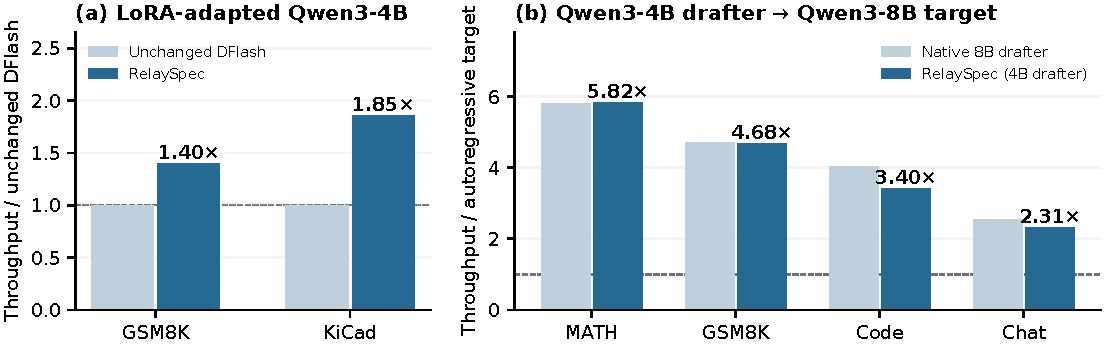
\includegraphics[width=\linewidth]{figures/relayspec_speedups.pdf}
    \caption{RelaySpec adapts a frozen drafter to a changed target. (a) On LoRA-adapted Qwen3-4B targets, the maps raise mean per-request throughput by 39.51\% on GSM8K and 85.47\% on KiCad over the unchanged DFlash drafter. (b) A Qwen3-4B drafter reused with Qwen3-8B reaches 5.82$\times$ and 4.68$\times$ autoregressive throughput on MATH and GSM8K, with the native 8B drafter shown for comparison. The panels use different baselines. Fitting the maps took under six minutes in (a) and 25 minutes in (b), and no draft weight is updated. Section~\ref{sec:setup} gives the evaluation settings.}
    \label{fig:main-speedups}
\end{figure}

As Large Language Models (LLMs) continue to advance, efficient inference remains a challenge. Autoregressive decoding generates one token at a time. This inherent seriality creates a major performance bottleneck: decoding is slow, memory-bound, and fails to fully utilize modern GPUs~\citep{cai2024medusa,vaswani2017attention}.

Speculative decoding accelerates a language model, called the \emph{target}, using a smaller model or prediction module, called the \emph{drafter}. The drafter proposes several candidate tokens, and the target checks them in parallel, keeping an accepted prefix and replacing the first rejected proposal with a correction. Appropriate acceptance and correction rules preserve the target's output distribution~\citep{leviathan2023speculative,chen2023sampling}, an idea that goes back to blockwise parallel decoding~\citep{stern2018blockwise} and now covers a broad family of methods~\citep{xia2024survey}. Speedup depends primarily on the length of the accepted prefix in each proposed block, together with the time spent drafting and verifying that block.

Some drafters also use the target's hidden-state representations, which provide contextual information that helps the drafter propose tokens the target will accept. Medusa adds parallel prediction heads to the target's final hidden states~\citep{cai2024medusa}, the EAGLE family uses target features to guide autoregressive drafting~\citep{li2024eagle,li2024eagle2,li2025eagle3}, and DFlash uses a block-diffusion drafter to predict several tokens in one pass, injecting fused target representations into every layer of the drafter model~\citep{chen2026dflash}. Other systems keep the drafter separate and restructure verification instead, using tree-based proposals~\citep{miao2024specinfer,chen2024sequoia}, Jacobi-style decoding~\citep{fu2024lookahead}, or layers of the target itself~\citep{zhang2024draftverify,elhoushi2024layerskip}.

This dependence complicates reuse of the drafter model when a service changes its target's size or family, or fine-tunes it using methods such as LoRA~\citep{hu2022lora}. The new target can produce different hidden states and preferred continuations, and changed feature dimensions may be incompatible with the existing drafter. Training a replacement drafter model requires target-specific supervision, optimization of the drafter's weights, and validation~\citep{li2025eagle3,chen2026dflash}. Repeating this process across target variants increases training and maintenance costs. Can we instead reuse an existing drafter by adapting only its target-feature inputs?

We introduce RelaySpec, a method for reusing a pretrained DFlash drafter~\citep{chen2026dflash} after its target changes (Figure~\ref{fig:relayspec-overview}). Section~\ref{sec:preliminaries} explains the parts of DFlash that RelaySpec uses. The new target supplies hidden states from five layers. A separate linear map transforms each stream before the drafter's original fusion projection combines them. The resulting context conditions the drafter transformer, which predicts a block of candidate tokens.

During adaptation, only the five maps are trained. The target, original fusion projection, drafter transformer, normalization layers, and the embeddings and output head selected for the model pair remain frozen. A map can be rectangular when the target and drafter expect different feature dimensions. Before inference, we multiply each map into its corresponding fusion block, a composition of linear operations. This produces one effective projection, so inference needs no separate mapping operation.

\begin{figure}[t]
    \centering
    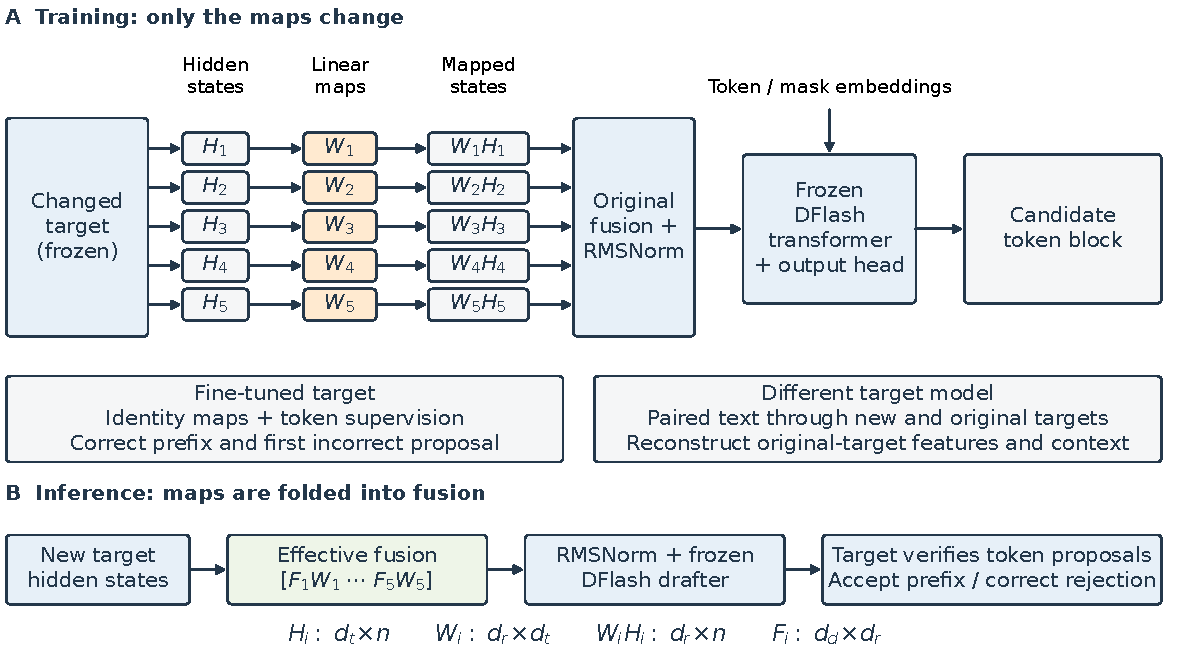
\includegraphics[width=\linewidth]{figures/relayspec_overview.pdf}
    \caption{RelaySpec training and inference. Orange maps are trainable and blue components are frozen. Each hidden-state matrix $H_i$ enters a map $W_i$ before fusion, and a single token gives $W_i h_{i,t}$. For Qwen3-8B with the Qwen3-4B drafter, $d_t=4096$ and $d_r=d_d=2560$, so each $W_i$ is $2560\times4096$ and the folded fusion projection is $2560\times20480$.}
    \label{fig:relayspec-overview}
\end{figure}

RelaySpec uses training signals that match the change in the feature interface: identity-initialized maps trained to improve the accepted prefix for a LoRA-fine-tuned target, and maps that reconstruct the original target's features and fused context for cross-model transfer. Section~\ref{sec:method} gives both procedures.

Our contributions are:
\begin{itemize}
    \item We introduce RelaySpec, an adapter layer between a target model's hidden-state representations and a pretrained DFlash drafter. It uses five trainable linear maps, keeps the drafter transformer frozen, and folds into the original fusion projection before inference.
    \item We evaluate adaptation across fine-tuned targets, model sizes and families, with training-budget and shared-serving comparisons. On Qwen3-4B LoRA targets the selected maps improve mean per-request throughput over the unchanged DFlash drafter by 39.51\% and 85.47\% on GSM8K~\citep{cobbe2021gsm8k} and KiCad. The selected Qwen3-4B-to-8B transfer recovers 100.2\% and 99.4\% of native-drafter throughput on MATH and GSM8K, with weaker transfer on code and chat.
    \item We analyze full-map and correction-map SVD truncation, correction scaling, alignment with LoRA-induced feature changes, and interpolation toward MSE-trained maps.
\end{itemize}



\section{Preliminaries}
\label{sec:preliminaries}
\label{sec:background}
\label{sec:dflash-background}
The \emph{original target} is the model used to train the available drafter, which we call the original target's \emph{native drafter}. The \emph{new target} is the model we want to accelerate.

DFlash predicts several future tokens in parallel~\citep{chen2026dflash}. At each decoding step it forms a block with the last token committed by the target, called the \emph{anchor}, followed by masked proposal positions. The released Qwen3-4B DFlash checkpoint has a default block size of 16, so each block contains one anchor and 15 proposals, and the reference generator defaults to temperature zero, so we use greedy decoding. One drafter pass predicts all 15 proposals and the target checks them in parallel. With greedy verification, speculative decoding is theoretically guaranteed to produce the same token sequence as greedy target-only decoding~\citep{leviathan2023speculative,chen2023sampling}.

DFlash also conditions the drafter on hidden-state representations from five fixed target layers. We use $d_t$ for the new target's hidden-state width, $d_r$ for the original target's width expected by the reused fusion projection, and $d_d$ for the drafter transformer's hidden width. Let $h^{(o)}_{i,t}\in\mathbb R^{d_r}$ be the original target's representation at token $t$ from layer $i$. The original fusion projection has five blocks $F_i\in\mathbb R^{d_d\times d_r}$, whose horizontal concatenation is $F=[F_1\;\cdots\;F_5]$. For one token, DFlash computes
\begin{equation}
 c^{(o)}_t=N\!\left(\sum_{i=1}^{5}F_i h^{(o)}_{i,t}\right)\in\mathbb R^{d_d},
 \label{eq:native-fusion}
\end{equation}
where $N$ is the original RMSNorm~\citep{zhang2019rmsnorm}. DFlash supplies this fused context as key and value entries to every transformer layer of the drafter~\citep{chen2026dflash,vaswani2017attention}, with the anchor and masked positions providing the queries; only target representations before the anchor are visible, so the drafter cannot access the tokens it is predicting.

RelaySpec adapts this interface. For $n$ tokens the new target supplies $H_i=[h_{i,1}\;\cdots\;h_{i,n}]\in\mathbb R^{d_t\times n}$ from layer $i$, and RelaySpec learns $W_i\in\mathbb R^{d_r\times d_t}$, mapping one vector to $W_i h_{i,t}\in\mathbb R^{d_r}$. The adapted context for one token is
\begin{equation}
 \hat c_t=N\!\left(\sum_{i=1}^{5}F_iW_i h_{i,t}\right)\in\mathbb R^{d_d},
 \label{eq:relayspec-fusion}
\end{equation}
and the maps fold into $G=[F_1W_1\;\cdots\;F_5W_5]\in\mathbb R^{d_d\times 5d_t}$. The fusion projection, RMSNorm, drafter transformer, token embedding and vocabulary head remain frozen. If the new target uses a different tokenizer, a separate vocabulary conversion is required.


\section{Related Work}
\label{sec:related-work}
\paragraph{Adapting and reusing drafters.}
EDA and RelaySpec both use target-specific training data, but EDA separates the drafter into shared and target-specific components and trains the lightweight private component, whereas RelaySpec trains five maps at DFlash's hidden-state input and leaves the drafter transformer unchanged~\citep{lin2026eda}. Online Speculative Decoding continually updates one or more drafters from observed serving queries, and OmniDraft adds an online n-gram cache, hybrid distillation, and vocabulary conversion, whereas RelaySpec trains its maps offline and performs no serving-time training~\citep{liu2024online,ramakrishnan2025omnidraft}. PARD trains a target-independent parallel drafter for a family of targets, and PARD-2 trains one drafter to support target-independent and target-conditioned modes, whereas RelaySpec starts from an already trained target-conditioned DFlash drafter and changes only its feature interface~\citep{an2026pard,an2026pard2}.

\paragraph{Adapting pretrained drafters through target features.}
SD$^2$ is the closest method-level comparison because it also conditions a pretrained drafter on target hidden states~\citep{berdoz2026steering}. Its main method injects a learned steering signal into every feed-forward layer and fully fine-tunes the autoregressive drafter, whereas RelaySpec maps the five feature streams already used by DFlash and keeps its transformer frozen. SD$^2$ also tests a frozen drafter, but its signal is still injected within every feed-forward layer, whereas RelaySpec places the maps before the existing fusion projection and folds them into that projection before inference.


\section{Method}
\label{sec:method}
RelaySpec reuses a pretrained speculative drafter when its target is fine-tuned or replaced by a different model. We train linear maps that transform the new target's hidden states into inputs the existing drafter can use, while keeping the target and the original drafter weights frozen. The drafter uses these mapped features to propose tokens, and the new target verifies them. This lets us adapt the drafter to a changed target without retraining its prediction network. Our main implementation and experiments use DFlash~\citep{chen2026dflash}, so we describe its architecture and training procedures first, then apply the same construction to EAGLE-3.

\subsection{Adapting the drafter's inputs}
\label{sec:method-inputs}
We retain the drafter's $K$ target-layer inputs and place one map before each original fusion block~\citep{chen2026dflash}, with $K=5$ for DFlash. Map $W_i$ connects the new target's feature stream $i$ to the corresponding drafter input and is applied at every token position. A bias-free $W_i\in\mathbb R^{d_r\times d_t}$ converts $h_{i,t}\in\mathbb R^{d_t}$ to the width $d_r$ the drafter expects, and the frozen fusion block $F_i\in\mathbb R^{d_d\times d_r}$ projects it to the draft width $d_d$. The $K$ streams give the context
\begin{equation}
 \widehat c_t=N\!\left(\sum_{i=1}^{K}F_i W_i h_{i,t}\right),
 \label{eq:mapped-context}
\end{equation}
where $N$ is the original RMSNorm~\citep{zhang2019rmsnorm}. Only $W_1,\ldots,W_K$ are trained; the target, fusion projection, normalization, draft transformer, token embeddings and vocabulary head all remain frozen.

After training, we multiply each learned matrix $W_i$ by its corresponding fusion block $F_i$ and join the $K$ products into one matrix:
\begin{equation}
 G=[F_1W_1\;\cdots\;F_KW_K]\in\mathbb R^{d_d\times Kd_t},
 \qquad \widehat c_t=N(G[h_{1,t};\ldots;h_{K,t}]).
 \label{eq:folded-fusion}
\end{equation}
Block multiplication gives $G[h_{1,t};\ldots;h_{K,t}]=\sum_i F_iW_ih_{i,t}$, so one multiplication by $G$ replaces the separate map and fusion operations in exact arithmetic, with the original normalization applied afterward (Figure~\ref{fig:relayspec-overview}). We keep the maps linear because a linear map both changes the feature width and folds into the fusion projection, and a nonlinear alternative with more parameters does not improve on it (Section~\ref{sec:ablations}).

\subsection{Training for a LoRA-adapted target}
\label{sec:method-auf}
\textbf{Initialization.} LoRA fine-tuning~\citep{hu2022lora} leaves the feature dimensions unchanged, so we initialize each map to the identity. Then $F_iW_ih_{i,t}=F_ih_{i,t}$ for every input, and inserting the maps does not disrupt the existing drafter's behavior with the adapted target; this preserves the starting behavior with the active LoRA target, not the behavior before fine-tuning. Training learns changes $\Delta_i=W_i-I$ that help the frozen drafter predict the adapted target's tokens.

\textbf{Training data.} We generate responses with the adapted target and save their tokens and hidden states. At sampled response positions the drafter receives one known token followed by 15 masked positions, matching the pretrained Qwen DFlash block of 16~\citep{chen2026dflash}, so we adapt the existing drafter without changing its prediction procedure. Each block sees target features only from before its starting position, and attention connects positions within a block but not separate blocks.

\textbf{Objective.} Because verification stops at the first rejected proposal, we supervise the correct prefix and the first incorrect prediction, excluding later positions: the accept-until-fail (AUF) objective~\citep{yang2026specauf}. For block $b$ and position $j$, with $q_{bj}$ the predicted distribution, $y_{bj}$ the saved target token and $m_{bj}$ a mask excluding padding and non-response positions,
\begin{equation}
 \begin{gathered}
 u_{bj}=\mathbf 1\!\left[\arg\max_v q_{bj}(v)=y_{bj}\ \text{or}\ m_{bj}=0\right],
 \qquad s_{bj}=\operatorname{stopgrad}\bigl({\textstyle\prod_{k<j}u_{bk}}\bigr),\\
 \mathcal L_{\mathrm{AUF}}
 =-\frac{\sum_{b,j}m_{bj}s_{bj}\log q_{bj}(y_{bj})}
 {\sum_{b,j}m_{bj}s_{bj}}.
 \end{gathered}
 \label{eq:auf-method}
\end{equation}
The product includes only earlier predictions, so the first failure still receives supervision. We recompute this mask from current predictions and hold it fixed during differentiation, gradients pass through the frozen drafter to update the maps, and we normalize the loss within each microbatch before averaging across accumulation steps and workers.

\subsection{Training for transfer across models}
\label{sec:method-mse}
\textbf{Initialization.} A drafter trained with one target expects that target's hidden states, and replacing the target changes both their dimensions and meaning. We therefore train the maps to reconstruct features from the original target, initializing them with independent Xavier-uniform values~\citep{glorot2010initialization}.

\textbf{Training data.} We generate responses with the new target, then run both targets causally on the same saved prompt and response to collect paired hidden states; the original target does not generate a separate response and is not used during adapted inference. With a shared tokenizer both receive identical token IDs, and when tokenizers differ we pair only positions corresponding to the same text prefix.

\textbf{Objective.} Let $h_{bti}$ and $h^{(o)}_{bti}$ be the paired new- and original-target features in stream $i$. The original features supply the context we reconstruct:
\begin{equation}
 c^{(o)}_{bt}=N\!\left(\sum_{i=1}^{K}F_i h^{(o)}_{bti}\right).
 \label{eq:original-context}
\end{equation}
For $B$ examples, let $S_b$ contain the selected valid prompt and response positions in example $b$. Using relative squared error, we minimize
\begin{gather}
 D(u,v)=\frac{\lVert u-v\rVert_2^2}{\lVert v\rVert_2^2+\varepsilon},
 \qquad \varepsilon=10^{-6},
 \label{eq:relative-error}\\
 \mathcal L_{\mathrm{MSE}}
 =\frac1B\sum_{b=1}^{B}\frac1{|S_b|}\sum_{t\in S_b}
 \left[\frac1K\sum_{i=1}^{K}D(W_i h_{bti},h^{(o)}_{bti})
 +D(\widehat c_{bt},c^{(o)}_{bt})\right].
 \label{eq:mse-method}
\end{gather}
The first term averages reconstruction errors across the $K$ feature streams and the second reconstructs the combined context received by the draft layers, with equal weight. We exclude padding and average positions within each example before averaging examples. Unlike AUF, this objective trains the maps without passing gradients through the draft transformer. Dividing by each original vector's squared norm makes the error relative to its magnitude. Reconstruction is a training objective, not a guarantee of accepted tokens, so we evaluate live decoding separately.

\subsection{Extension to EAGLE-3}
\label{sec:method-eagle}
The construction is not specific to DFlash. EAGLE-3 combines features from three target layers before autoregressive drafting~\citep{li2025eagle3}, so $K=3$. We place one map before each of those inputs, leave the original feature projection, prediction network and autoregressive drafting procedure unchanged, and fold the maps into that projection exactly as in Equation~\ref{eq:folded-fusion}. We pair each setting with the same objective we use for DFlash: identity initialization with token supervision for a LoRA-adapted target, applying the accept-until-fail rule along EAGLE-3's own recurrent path, and Xavier initialization with reconstruction for a replaced target. Appendix~\ref{app:eagle-method} gives the recurrent objective in full.

\subsection{Generation and verification}
\label{sec:method-generation}
The new target computes hidden states during prompt processing and proposal verification. We retain states from the committed prefix and map them into context for subsequent drafting. The frozen drafter proposes tokens, and the target verifies them using its existing decoding procedure. After verification, the decoder removes rejected speculative positions from the caches before the next drafting step. The original target is no longer needed to supply features during generation. Cross-tokenizer transfer additionally requires a proposal-conversion procedure, which the hidden-state maps do not provide.

Under greedy decoding, changing the drafter does not change the target's output provided block verification makes the same choices as sequential target evaluation on identical prefixes; Appendix~\ref{app:greedy} gives the argument and its assumptions.



\section{Experiments}
\label{sec:experiments}
\subsection{Experimental setup}
\label{sec:setup}

\textbf{Models and references.} Every DFlash experiment starts from one pretrained checkpoint released for Qwen3-4B~\citep{chen2026dflash,yang2025qwen3}; Section~\ref{sec:eagle} additionally uses published EAGLE-3 checkpoints, which read three streams~\citep{li2025eagle3}. No draft transformer is ever trained. In the \emph{fine-tuned} setting the target carries a LoRA adapter the released drafter has never seen~\citep{hu2022lora}: Qwen3-4B with a GSM8K, KiCad or NanoCoder adapter, and Qwen3-8B with a GSM8K or CodeAlpaca~\citep{chaudhary2023codealpaca} adapter. In the \emph{replaced} setting we evaluate four transfers, named by the target they accelerate and the model the drafter came from: Qwen3-8B from Qwen3-4B, Qwen3-4B from Qwen3-8B, Llama3.1-8B from Qwen3-4B, and Llama3.2-3B from Llama3.1-8B~\citep{grattafiori2024llama3}; only the third has mismatched tokenizers and uses the proposal bridge of Section~\ref{sec:method-generation}. Maps are $2560\times2560$ when the target keeps the drafter's feature width (32.8M parameters) and $2560\times4096$ for Qwen3-8B (52.4M). For a fine-tuned target the reference is the \emph{unadapted drafter}, the released checkpoint run with no adaptation, because that is what a deployment would otherwise use; for a replaced target it is the \emph{native drafter}, one trained for the target being accelerated.

\textbf{Metrics.} \emph{Speedup} is mean per-request throughput divided by that of autoregressive decoding of the same target on the same prompts, so autoregressive decoding is $1.00\times$ by definition. \emph{Acceptance length} $\tau$ is pooled emitted tokens per verification step including the correction token. Aggregate serving throughput divides total returned tokens by workload wall time including drain. These statistics weight requests differently and we never mix them inside one comparison. Where an ablation must choose one configuration we select by the harmonic mean of its per-workload speedups, because the harmonic mean of ratios is pulled down by the smallest entry and will not let a configuration hide one weak workload behind a favourable average.

\textbf{Data and implementation.} Transfer experiments use MATH test~\citep{hendrycks2021math}, GSM8K test~\citep{cobbe2021gsm8k}, pinned LiveCodeBench releases~\citep{jain2024livecodebench} and single-turn UltraFeedback instructions~\citep{cui2024ultrafeedback}, reported as Math, GSM8K, Code and Chat; fine-tuned experiments use held-out prompts from the adapter's own domain. Every cell uses 128 held-out prompts with a 2{,}048-token cap, except KiCad at 8{,}192. Fine-tuned fits use 4{,}096 target-generated responses, 32 anchors per example and one epoch, 512 updates at global batch 8 with AdamW~\citep{loshchilov2019adamw} at learning rate $10^{-4}$; transfer fits reuse 16{,}384 saved NuminaMath~\citep{li2024numinamath} trajectories at 25\% position coverage for three epochs, 6{,}144 updates at learning rate $10^{-3}$. Both use seed 42 on two L40S GPUs with FP32 trainable maps over a frozen BF16 model. Single-request measurements use Transformers~\citep{wolf2020transformers} with greedy non-thinking decoding; serving uses vLLM 0.28.0~\citep{kwon2023vllm} with batch-invariant operations and FlashAttention~\citep{dao2023flashattention2}, and stacks such as SGLang~\citep{zheng2024sglang} differ. In the selected single-request comparisons all drafters returned identical output sequences on all 128 prompts. Appendix~\ref{app:setup-full} gives the remaining detail.

\subsection{Main results}
\label{sec:main-results}
Table~\ref{tab:main} reports every target, workload and reference in one place. Two conclusions follow from it.

\begin{table}[t]
\centering
\caption{Complete single-request results. AR is the measured autoregressive tokens per second for that target on that workload, the common $1.00\times$ baseline for every speedup in the row. Speedup is mean per-request throughput divided by AR. $\tau$ is average acceptance length including the correction token. The reference for a fine-tuned target is the released drafter used with no adaptation, so $\times$ref above 1 is an improvement over what a deployment would otherwise run. The reference for a replaced target is a drafter trained for that target, so $\times$ref near 1 means RelaySpec matches target-specific drafter training without performing any. A target written $A\leftarrow B$ is target $A$ accelerated by a drafter built for $B$. Bold marks $\times$ref at or above parity.}
\label{tab:main}
\small
\setlength{\tabcolsep}{4.2pt}
\begin{tabular}{llrrrrrr}
\toprule
& & & \multicolumn{2}{c}{RelaySpec} & \multicolumn{2}{c}{Reference drafter} & \\
\cmidrule(lr){4-5}\cmidrule(lr){6-7}
Target $\leftarrow$ drafter & Workload & AR & Speedup & $\tau$ & Speedup & $\tau$ & $\times$ref \\
\midrule
\multicolumn{8}{l}{\emph{Fine-tuned target. Reference is the released drafter, used unadapted.}} \\
Qwen3-4B + GSM8K LoRA & GSM8K & 38.81 & 4.63$\times$ & 5.99 & 3.32$\times$ & 4.47 & \textbf{1.40} \\
Qwen3-4B + KiCad LoRA & KiCad & 38.42 & 8.13$\times$ & 11.26 & 4.39$\times$ & 5.99 & \textbf{1.85} \\
Qwen3-4B + NanoCoder LoRA & NanoCoder & 39.01 & 4.40$\times$ & 5.55 & 3.87$\times$ & 5.11 & \textbf{1.14} \\
Qwen3-8B + GSM8K LoRA & GSM8K & 37.89 & 4.59$\times$ & 6.35 & 3.40$\times$ & 4.76 & \textbf{1.35} \\
Qwen3-8B + CodeAlpaca LoRA & CodeAlpaca & 37.56 & 4.32$\times$ & 5.63 & 4.07$\times$ & 5.62 & \textbf{1.06} \\
\midrule
\multicolumn{8}{l}{\emph{Replaced target. Reference is a drafter trained for the target being accelerated.}} \\
Qwen3-8B $\leftarrow$ Qwen3-4B & Math & 37.84 & 5.82$\times$ & 7.98 & 5.81$\times$ & 8.21 & \textbf{1.00} \\
 & GSM8K & 37.76 & 4.68$\times$ & 6.24 & 4.71$\times$ & 6.48 & 0.99 \\
 & Code & 37.50 & 3.40$\times$ & 4.74 & 4.04$\times$ & 5.64 & 0.84 \\
 & Chat & 35.09 & 2.31$\times$ & 2.89 & 2.55$\times$ & 3.32 & 0.90 \\
\addlinespace[1pt]
Qwen3-4B $\leftarrow$ Qwen3-8B & Math & 39.42 & 5.49$\times$ & 7.66 & 5.70$\times$ & 8.09 & 0.96 \\
 & GSM8K & 39.72 & 4.27$\times$ & 5.99 & 4.46$\times$ & 6.34 & 0.96 \\
 & Code & 39.60 & 3.30$\times$ & 4.89 & 4.34$\times$ & 6.26 & 0.76 \\
 & Chat & 40.48 & 2.01$\times$ & 2.83 & 2.36$\times$ & 3.36 & 0.85 \\
\addlinespace[1pt]
Llama3.1-8B $\leftarrow$ Qwen3-4B & Math & 41.00 & 2.97$\times$ & 4.63 & 3.17$\times$ & 5.12 & 0.94 \\
 & GSM8K & 41.11 & 2.21$\times$ & 3.23 & 3.10$\times$ & 4.42 & 0.71 \\
 & Code & 40.79 & 1.98$\times$ & 3.05 & 3.00$\times$ & 4.52 & 0.66 \\
 & Chat & 40.96 & 1.48$\times$ & 2.06 & 2.79$\times$ & 3.95 & 0.53 \\
\bottomrule
\end{tabular}
\setlength{\tabcolsep}{6pt}
\end{table}

\textbf{Adapting a fine-tuned target's features recovers a large share of lost drafting quality.} Training only the five maps improves every adapter at both target scales, from $+6\%$ on CodeAlpaca to $+85\%$ on KiCad, and raises acceptance length in every cell. The gain tracks acceptance: KiCad nearly doubles acceptance length, 5.99 to 11.26, reaching $8.13\times$ autoregressive throughput, whereas CodeAlpaca moves from 5.62 to 5.63 and gains little.

\textbf{A drafter can be moved to a different target model and still approach one built for it.} Every transfer accelerates its target on every workload. Within the Qwen3 family the maps reach $1.002\times$ and $0.994\times$ of a native drafter on Math and GSM8K when moving up in scale, with no target-specific drafter training; recovery is lower on Code and Chat, and lower again across families, so the setting is effective within a family and partial across one. A fifth transfer, a Llama3.1-8B drafter reused for Llama3.2-3B, reaches $2.35\times$ autoregressive throughput on Math and above $1.6\times$ on every workload (Appendix~\ref{app:llama-table}).

\subsection{Ablation studies}
\label{sec:ablations}
We ablate the three decisions that define the method. Appendix~\ref{app:ablations} reports all of them in full.

\textbf{Where the trained parameters sit.} Training one matrix of the same total size in place of the five maps, initialized to exactly the function the five maps start from, reaches a harmonic mean of 1.265 against 1.376 for the five maps and loses 45 points of gain on KiCad; transferring to Qwen3-8B it reaches $0.365\times$ the native drafter on Math while the five maps reach $0.884\times$. The factorization does the work, not the parameter count, which is the behaviour structural re-parameterization predicts~\citep{huo2026repspec}. Low-rank replacement of each whole map degrades monotonically. Draft-transformer LoRA is competitive and wins on NanoCoder, so we do not claim input adaptation beats body adaptation on every workload; its cost is that the draft transformer is no longer shared.

\textbf{Which objective trains the maps.} For a fine-tuned target the two token objectives are nearly tied on the arithmetic mean, 1.451 against 1.445, but the harmonic mean separates them, 1.376 for accept-until-fail against 1.353 for decaying cross-entropy, because it refuses to let the 1.031 NanoCoder entry be averaged away. Reconstruction on the same targets reaches only 1.052. For a replaced target the ordering reverses and becomes decisive: both reconstruction variants exceed 0.918 while the best token objective reaches 0.623, the gap coming almost entirely from Code and Chat where token supervision collapses to 0.406 and 0.573. We therefore select accept-until-fail for fine-tuned targets and reconstruction for replaced ones, and the pairing does real work in both directions (Appendix~\ref{app:objective-table}).

\textbf{Whether the maps need to be nonlinear.} Adding a parallel branch so stream $i$ contributes $W_ih_i+B_i\operatorname{SiLU}(A_ih_i)$~\citep{elfwing2018silu}, with $B_i$ initialized to zero so training starts at exactly the linear solution, changes throughput by between $-2.07\%$ and $+2.97\%$, leaves acceptance length almost unchanged, and is behind the linear map on five of seven workloads while carrying 16 to 20 percent more parameters and remaining an active computation at inference.

\textbf{How much supervision the maps need.} Adaptation is effective from as few as 16 examples, and throughput rises smoothly without saturating out to 16{,}384: GSM8K goes from $+10.8\%$ to $+45.0\%$ and KiCad from $+5.0\%$ to $+113.0\%$, while transfer recovery rises from 15.6\% to 99.9\% on Math and 18.9\% to 84.8\% on Code (Appendix Figure~\ref{fig:scaling}). The main results are therefore conservative operating points rather than ceilings.

\subsection{Generalization, comparison and cost}
\label{sec:eagle}
\textbf{A second drafter family.} We repeat both settings on published EAGLE-3 checkpoints, which read three target streams and draft one token at a time, pairing each setting with the objective selected above. Adapting the inputs of a frozen EAGLE-3 drafter improves it in both settings, by 45.9\% to 105.7\% on fine-tuned targets and above a purpose-built Qwen3-8B EAGLE-3 drafter on all four transfer workloads (Appendix~\ref{app:eagle-table}). Against autoregressive decoding of the same fine-tuned target it reaches $3.82\times$, $3.75\times$ and $5.00\times$ on GSM8K, NanoCoder and KiCad, against $2.26\times$, $2.57\times$ and $2.43\times$ unadapted. The objective selection also replicates: training the same three maps by reconstruction instead gives 71.89, 75.34 and 78.70 tokens per second, a 7.9\% regression on NanoCoder, while token supervision gives 120.35, 119.30 and 151.86 on the same prompts. Pairing the objective to the setting is therefore not a DFlash artifact.

\textbf{Published systems, serving and cost.} An earlier single-projection version of this interface, compared on the same 128 MATH development questions against PARD~\citep{an2026pard} and frozen-drafter SD$^2$~\citep{berdoz2026steering} with each measured against its own runtime's autoregressive baseline, reaches $5.14\times$ [4.90, 5.37] against $3.34\times$ and $1.60\times$ (Appendix~\ref{app:public-runtime}). Under vLLM with three LoRA targets sharing one draft backbone, aggregate server throughput is higher for the adapted drafter at every concurrency, reaching 4{,}324 tokens per second against 2{,}440 unadapted and 828 autoregressive at 32 clients, one pooled set of maps reaches 98.9--99.6\% of three separate sets, and adaptation adds a constant 0.33 GiB. Against the published DFlash recipe of about 800{,}000 samples for six epochs~\citep{chen2026dflash}, our recipes use 4{,}096 and 16{,}384 examples, about 195 and 49 times fewer, each fitting in under half an hour on two GPUs (Appendix~\ref{app:ablations}).


\section{Analysis}
\label{sec:analysis}
We analyze how the learned maps change the hidden-state context passed to the frozen drafter. Appendix~\ref{app:analysis-probes} reports every measurement, control and negative result.

\subsection{What changes when the interface already works?}
\label{sec:analysis-lora}
For a LoRA-fine-tuned target, identity maps recover the native DFlash interface. Write $z_0=\sum_i F_i h_i$ for this context and $\delta=\sum_i F_i(W_i-I)h_i$ for the correction. Running decoding with $z_0$ plus only the component of $\delta$ parallel to $z_0$ returns acceptance length to the native level, 4.466 against 4.472 tokens per verification step on GSM8K, while the perpendicular component alone recovers nearly all of the full map's acceptance length, 5.924 against 5.988 (Appendix~\ref{app:lora-direction}). Scaling the whole context by two leaves acceptance length unchanged. The useful change is mainly directional, consistent with RMSNorm suppressing common rescaling.

Do the maps reverse the change caused by LoRA fine-tuning? Comparing the correction with the LoRA-induced change in fused context on 1,024 positions, with the LoRA changes shuffled as a control, gives a mean cosine of $-0.0429$ on GSM8K and $0.1248$ on NanoCoder against shuffled $-0.0413$ and $0.1052$ (Appendix~\ref{app:lora-geometry}). The maps therefore redirect an already usable context rather than recovering the pre-LoRA one. Identity-preserving SVD keeps most of the benefit at moderate rank, with rank 128 on GSM8K retaining 5.928 against 5.988, whereas truncating the whole map to rank 1 or 2 removes the identity path and collapses drafting performance.

\subsection{Why does reconstruction help across model sizes?}
\label{sec:analysis-transfer}
We study a Qwen3-8B target with a pretrained Qwen3-4B drafter, where MSE reconstructs the corresponding Qwen3-4B features while AUF and decay CE train through token predictions, all from the same Xavier initialization. MSE recovers the interface the frozen drafter was built for: its normalized context error is 0.136 against 0.940 for AUF and 0.900 for decay CE, and its per-stream source cosine is 0.944--0.985 against 0.121--0.279 (Appendix~\ref{app:transfer-geometry}). This transfers to prediction: on held-out positions where only the maps differ, MSE gives the lowest cross-entropy and longest correct prefix on MATH, Code and Chat (Appendix~\ref{app:heldout-diagnostics}), and averaging each token-trained map with its MSE counterpart improves live throughput and acceptance without retraining (Appendix~\ref{app:midpoint-full}). Initialization does not explain this: retraining from a rectangular identity leaves MSE acceptance nearly unchanged on MATH and GSM8K and lowers its throughput on all four workloads, while AUF and decay CE improve on both yet stay below MSE (Appendix~\ref{app:identity-init}).


\section{Conclusion}
\label{sec:conclusion}
RelaySpec trains one linear map per target feature stream, keeps the drafter frozen, and folds the maps into the existing fusion projection, so inference runs the original architecture with one updated matrix. It improves every fine-tuned adapter we tested and recovers a purpose-built native drafter within a model family from as little as 16 examples.


% Statements below are outside the main-text page limit.
% AI disclosure is required. Ethics and reproducibility are recommended.
\subsection*{AI Use Statement}
We used large language model assistants for code support and for editing prose. Assistants helped write and debug experiment, evaluation and figure-generation scripts, and helped revise wording and structure in this manuscript. All research questions, experimental designs, model and data choices, and claims are the authors'. Every number reported here comes from our own recorded measurements, and the authors verified each claim against those records. The authors take full responsibility for the content of this paper, including any remaining errors.


\subsection*{Ethics Statement}
This work studies inference efficiency for existing language models. It does not train or release a new target model, does not change any target's output distribution under greedy verification, and does not introduce new capabilities or new training data about people. All targets, drafters and datasets are publicly released artifacts used under their own licenses, and the domain adapters we evaluate come from previously released checkpoints.

The main societal consideration is indirect. Faster inference lowers the cost of deploying language models, which amplifies both their benefits and any harms of the underlying target model. RelaySpec inherits whatever behavior, bias or failure mode its target already has, and speculative decoding provides no additional safety property. Because adaptation is cheap, it also lowers the cost of maintaining many specialized target variants, which makes the provenance of each adapter worth tracking in a deployment. We report negative and partial results, including the workloads and model pairs where the method does not reach a native drafter, so that the method's limits are visible to anyone considering it.


\subsection*{Reproducibility Statement}
Section~\ref{sec:setup} states the drafter and target checkpoints, adapter sources, feature layer indices, map shapes and trained parameter counts, the training data and schedules for both settings, and the decoding, hardware and backend configuration used for every measurement. Section~\ref{sec:method} gives the exact objectives, including the accept-until-fail support mask and the relative reconstruction error with its normalization and epsilon. Every reported cell uses 128 held-out prompts, and the response caps are stated per workload.

The appendix reports the complete measurements behind every analysis claim in Section~\ref{sec:analysis}, including matching controls, all tested variants, negative results, metric definitions and units, and the timing repeats that bound run-to-run variation. Where a comparison comes from a separate cohort, a different architecture or a different learning rate, we state that alongside the numbers rather than presenting it as a matched ablation. Figures~\ref{fig:scaling} and~\ref{fig:serving} are generated directly from the recorded measurement tables by scripts released with the manuscript source, and the plotted values are saved alongside them.

Throughput measurements depend on hardware, backend version and batching, so absolute tokens per second should be expected to move across environments. The ratios we report are computed within a single environment against a control measured in that same environment, which is the comparison we intend to be reproducible.


\bibliography{references}
\bibliographystyle{iclr2027_conference}

% Appendices follow the references. Add headings when content is written.
\appendix
\section{Additional experimental detail and ablations}
\label{app:ablations}

\subsection{Remaining setup detail}
\label{app:setup-full}
Under vLLM the returned sequences can diverge from the single-request runs, consistent with documented numerical and batching variability, and we treat those numbers as descriptive rather than as exact-equivalence evidence. Fitting time throughout excludes response generation, feature capture, model setup and export. One saved feature cache serves several fits, so its cost must not be charged to each fit separately.

\subsection{Where the trained parameters sit}
\label{app:placement}

\subsubsection{Where the trained parameters sit}
\label{sec:ablation-placement}
RelaySpec trains one map per feature stream and then folds those maps into the fusion block in front of which they sit. Because the folded result is a single matrix, the natural objection is that the factorization is irrelevant and any trainable matrix of the same size would do. Table~\ref{tab:ablation-placement} tests that, against four alternatives:

\begin{itemize}\itemsep1pt\parskip0pt
\item \textbf{Single fused projection.} One matrix of the same total size, trained in place of the five maps and initialized to exactly the function the five maps start from. This is the decisive control, since it differs from RelaySpec only in being unfactorized.
\item \textbf{Draft-transformer LoRA.} A rank-128 LoRA on the attention and MLP projections inside the draft blocks. This trains the drafter's body instead of its inputs, and is the established alternative that RelaySpec is meant to replace.
\item \textbf{Single joint map.} One dense matrix over all five concatenated streams, which permits mixing between streams at five times the parameters.
\item \textbf{Rank-$r$ maps.} Each whole map is replaced by a rank-$r$ product, rather than adding a low-rank correction to a retained full map.
\end{itemize}

\begin{table}[t]
\centering
\caption{Where the trained parameters sit, for fine-tuned Qwen3-4B targets under a matched accept-until-fail objective, 4{,}096 examples and 32 anchors. Values are percent gain in mean throughput over the unadapted drafter. HM is the harmonic mean of the corresponding speedup ratios and is the selection criterion. Best in each column in bold.}
\label{tab:ablation-placement}
\small
\begin{tabular}{lrrrrr}
\toprule
Trained object & Parameters & GSM8K & KiCad & NanoCoder & HM \\
\midrule
Five per-stream maps (RelaySpec) & 32.8M & $\mathbf{+37.6}$ & $+89.5$ & $+8.1$ & \textbf{1.376} \\
Single fused projection & 32.8M & $+32.4$ & $+44.5$ & $+8.2$ & 1.265 \\
Draft-transformer LoRA, rank 128 & 36.7M & $+36.4$ & $+75.5$ & $\mathbf{+9.8}$ & 1.355 \\
Single joint map over all streams & 163.8M & $+24.3$ & $\mathbf{+88.4}$ & $-7.0$ & 1.244 \\
Rank-128 maps & 3.3M & $+3.2$ & $+58.4$ & $-28.8$ & 0.999 \\
Rank-56 maps & 1.4M & $-21.9$ & $+35.1$ & $-49.3$ & 0.751 \\
Rank-28 maps & 0.7M & $-43.1$ & $+12.8$ & $-62.5$ & 0.565 \\
\bottomrule
\end{tabular}
\end{table}

\textbf{What this shows.} For scale, the unadapted drafter used as the 0\% reference here already reaches $3.3\times$ to $4.4\times$ autoregressive decoding before any adaptation (Table~\ref{tab:main}), so every percentage below is the further gain adaptation adds on top of that autoregressive speedup, not the whole story. The factorization does the work, not the parameter count. With identical parameters and an identical starting function, the single fused projection reaches a harmonic mean of 1.265 against 1.376 for the five maps and loses 45 points of gain on KiCad. The same contrast appears when transferring to Qwen3-8B, where under a matched objective the single fused projection reaches $0.365\times$ the native drafter on Math while the five maps reach $0.884\times$. Keeping one map per stream therefore changes what the optimizer can reach, even though the two parameterizations describe the same functions after folding and export as the same matrix. This is the behaviour that structural re-parameterization predicts, where a training-time factorization that merges away at inference still improves the trained result~\citep{huo2026repspec}. Replacing each whole map by a low-rank product degrades monotonically, and the two smallest ranks fall below the unadapted drafter, because replacing the map discards its ability to pass the original feature through rather than merely limiting the learned correction. Draft-transformer LoRA is competitive and wins on NanoCoder, so we do not claim that adapting inputs beats adapting the body on every workload. Its cost is that the draft transformer is no longer shared, which Section~\ref{sec:serving} shows is what makes the method useful in deployment.

\subsection{Whether the maps need to be nonlinear}
\label{app:capacity}

\subsubsection{Whether the maps need to be nonlinear}
\label{sec:ablation-capacity}
The maps are linear because a linear map changes the feature width and still folds into the fusion projection. To test whether that costs accuracy, we add a parallel nonlinear branch to each map, so stream $i$ contributes $W_ih_i+B_i\operatorname{SiLU}(A_ih_i)$~\citep{elfwing2018silu}, with $A_i$ reducing to 256 coordinates and $B_i$ initialized to zero. Training therefore starts at exactly the linear solution and departs from it only if that lowers the loss. The branch raises trained parameters from 32.8M to 39.3M for a fine-tuned target and from 52.4M to 60.9M for transfer, and unlike the linear map it cannot be folded away before inference. Table~\ref{tab:ablation-capacity} holds data, objective and schedule fixed within each setting.

\begin{table}[t]
\centering
\caption{Whether the maps need to be nonlinear. Values are mean tokens per second and acceptance length under matched data, objective and schedule. The nonlinear alternative carries 16 to 20 percent more parameters and remains an active computation at inference. Best in each row in bold.}
\label{tab:ablation-capacity}
\small
\begin{tabular}{llrrrrr}
\toprule
& & \multicolumn{2}{c}{Tokens/s} & & \multicolumn{2}{c}{$\tau$} \\
\cmidrule(lr){3-4}\cmidrule(lr){6-7}
Setting & Workload & Linear & Nonlinear & Change & Linear & Nonlinear \\
\midrule
Fine-tuned & GSM8K & \textbf{179.83} & 177.94 & $-1.05\%$ & \textbf{5.988} & 5.953 \\
 & KiCad & 312.47 & \textbf{321.76} & $+2.97\%$ & 11.256 & \textbf{11.411} \\
 & NanoCoder & \textbf{171.73} & 169.74 & $-1.16\%$ & \textbf{5.552} & 5.520 \\
\midrule
Replaced & Math & \textbf{220.26} & 215.71 & $-2.07\%$ & \textbf{7.984} & 7.980 \\
 & GSM8K & \textbf{176.87} & 174.56 & $-1.31\%$ & 6.242 & \textbf{6.257} \\
 & Code & 127.61 & \textbf{128.41} & $+0.63\%$ & 4.739 & \textbf{4.782} \\
 & Chat & \textbf{80.93} & 80.78 & $-0.20\%$ & 2.887 & \textbf{2.902} \\
\bottomrule
\end{tabular}
\end{table}

\textbf{What this shows.} The nonlinear branch is given every advantage, since it starts from the linear solution, carries more parameters and is selected by the optimizer only if it lowers the loss. It nevertheless changes throughput by between $-2.07\%$ and $+2.97\%$, leaves acceptance length almost unchanged, and is behind the linear map on five of the seven workloads. The linear form is therefore not a concession made for foldability. It is at least as accurate here and additionally collapses to one fixed matrix before inference. With differences of this size and one timed pass per cell we claim only that this nonlinear interface does not pay for itself.

\subsection{Two further objective controls}
\label{app:objective-extra}
First, on a separate matched architecture (a single low-rank fusion update rather than the five per-stream maps, held fixed to isolate the loss), plain uniform cross-entropy, the DFlash decaying weighting, and accept-until-fail were compared under identical data and schedule on NanoCoder: accept-until-fail reaches $1.072\times$ autoregressive decoding against $1.046\times$ for uniform cross-entropy and $1.047\times$ for decaying cross-entropy, a $2.4\%$ gain over uniform weighting that decaying weighting does not reproduce. This confirms that the prefix-aware accept-until-fail weighting, not merely having some position-dependent weighting, is what improves throughput. Second, for a fine-tuned target the training responses do not need to come from the fine-tuned target itself: fitting the same architecture from the base model's own generations reaches $1.001\times$ the throughput of fitting from the fine-tuned target's generations on the fine-tuned target's evaluation prompts, with a paired 95\% interval of $[0.995, 1.007]$ that contains 1. The gain therefore reflects adaptation to the workload distribution rather than a fit to the fine-tuned target's specific outputs.

\subsection{Serving many targets from one drafter}
\label{sec:serving}
Because the draft transformer is never trained, several adapted targets can share one copy of it, with only a small matrix differing between them. This is what draft-transformer LoRA gives up. Figure~\ref{fig:serving} measures the deployment on a vLLM server holding one target backbone and one draft backbone with three LoRA targets and frozen route assignments.

\begin{figure}[t]
    \centering
    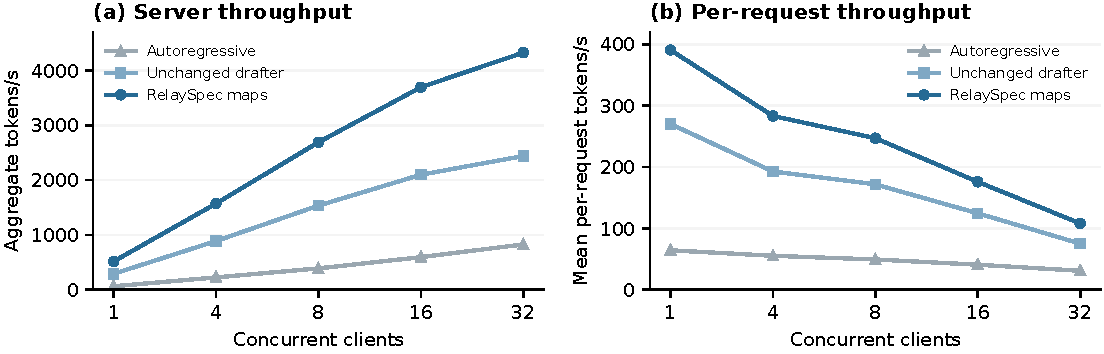
\includegraphics[width=\linewidth]{figures/relayspec_serving.pdf}
    \caption{One Qwen3-4B target backbone and one draft backbone serving three LoRA targets under vLLM on a single L40S, 384 requests with frozen route assignments. (a) aggregate throughput, total returned tokens divided by workload wall time including drain. (b) mean per-request throughput. The adapted drafter leads on server throughput at every concurrency, while per-request throughput falls with load for all three methods.}
    \label{fig:serving}
\end{figure}


\textbf{What this shows.} The single-request gains survive batching. Aggregate server throughput is higher for the adapted drafter at every concurrency measured, reaching 4{,}324 tokens per second against 2{,}440 for the unadapted drafter and 828 for autoregressive decoding at 32 clients, while acceptance length stays near 10.5 against 5.8. Panel (b) shows why both conventions must be reported: mean per-request throughput falls with load for all three methods even as server throughput rises, so a per-request number cannot stand in for a serving number. One pooled set of maps trained on the union of three domains reaches 98.9\% to 99.6\% of three separately trained sets across two repeats, so a deployment need not even hold one adapter per target. This is the practical form of the reuse question that motivates target-independent drafting~\citep{an2026pard2}. The advantage is not unbounded: on a Qwen3-8B server the adapted drafter leads at 1, 4 and 8 clients but falls within 4\% of the native drafter at 16 and 32 clients, because at high concurrency the bottleneck moves away from acceptance length.

\textbf{Concurrent serving across transfers.} The same question arises for a replaced target: does the transferred drafter still help once requests are batched under vLLM? Table~\ref{tab:transfer-serving} reports aggregate throughput at 16 concurrent clients for the three transfers with a published native drafter. Batching reproduces the single-request ordering of Table~\ref{tab:main} rather than changing it. On the transfer with the strongest single-request recovery, Qwen3-8B accelerated by the Qwen3-4B drafter, the mapped drafter leads on Math and GSM8K and trails narrowly on Code and Chat. On the reverse and cross-family transfers, where single-request recovery was already weaker, the mapped drafter trails the native drafter under concurrency on every workload, most on the cross-family Llama3.1-8B transfer. On the Llama3.2-3B transfer of Table~\ref{tab:llama-transfer}, the same server configuration reaches $2.53\times$, $3.08\times$, $1.71\times$ and $1.77\times$ autoregressive throughput on Math, GSM8K, Code and Chat at 16 clients.

\begin{table}[t]
\centering
\caption{Aggregate vLLM throughput at 16 concurrent clients, total returned tokens divided by workload wall time including drain. Bold marks the higher of native and mapped.}
\label{tab:transfer-serving}
\small
\begin{tabular}{llrrr}
\toprule
Target $\leftarrow$ drafter & Workload & Native (tok/s) & Mapped (tok/s) & Mapped/native \\
\midrule
Qwen3-8B $\leftarrow$ Qwen3-4B & Math & 2524.31 & \textbf{2716.26} & 1.076 \\
 & GSM8K & 2207.43 & \textbf{2262.03} & 1.025 \\
 & Code & \textbf{1748.19} & 1548.47 & 0.886 \\
 & Chat & \textbf{1091.14} & 1065.93 & 0.977 \\
\midrule
Qwen3-4B $\leftarrow$ Qwen3-8B & Math & \textbf{4482.42} & 3710.76 & 0.828 \\
 & GSM8K & \textbf{3160.99} & 3078.87 & 0.974 \\
 & Code & \textbf{2840.15} & 2002.79 & 0.705 \\
 & Chat & \textbf{1888.69} & 1431.21 & 0.758 \\
\midrule
Llama3.1-8B $\leftarrow$ Qwen3-4B & Math & \textbf{1894.99} & 1046.94 & 0.553 \\
 & GSM8K & \textbf{1354.50} & 853.13 & 0.630 \\
 & Code & \textbf{1296.83} & 636.97 & 0.491 \\
 & Chat & \textbf{1440.04} & 524.40 & 0.364 \\
\bottomrule
\end{tabular}
\end{table}

\textbf{Memory and GPU usage.} We measured post-request allocated and reserved GPU memory on the same T1 serving cells above. Allocated memory rises from 30.5914 GiB for the native drafter to 30.9190 GiB for the mapped drafter, a constant 0.33 GiB increase regardless of workload or concurrency; reserved memory shows the same small, workload-independent gap. This matches expectation: the trained maps add 52.4 million BF16 parameters to an 8-billion-parameter target and a several-billion-parameter draft transformer, so the memory cost of adaptation is negligible relative to the models it accelerates, and it does not grow with client count.

\subsection{EAGLE-3 generalization}
\label{app:eagle-table}
\begin{table}[t]
\centering
\caption{Generalization to EAGLE-3, using three input maps. Token supervision is used for a fine-tuned target and reconstruction for a replaced one, following the selection in Section~\ref{sec:ablation-objective}. The reference is the unadapted EAGLE-3 drafter for the fine-tuned block and a published EAGLE-3 drafter native to Qwen3-8B for the replaced block. Best in each row in bold. Acceptance uses EAGLE-3's upstream counters and is not comparable with the DFlash tables.}
\label{tab:eagle}
\small
\begin{tabular}{llrrrrr}
\toprule
& & \multicolumn{2}{c}{Tokens/s} & & \multicolumn{2}{c}{$\tau$} \\
\cmidrule(lr){3-4}\cmidrule(lr){6-7}
Setting & Workload & Reference & RelaySpec & $\times$ref & Reference & RelaySpec \\
\midrule
Fine-tuned Qwen3-4B, & GSM8K & 71.19 & \textbf{120.35} & \textbf{1.69} & 3.347 & \textbf{5.695} \\
token supervision & NanoCoder & 81.77 & \textbf{119.30} & \textbf{1.46} & 3.852 & \textbf{5.668} \\
 & KiCad & 73.82 & \textbf{151.86} & \textbf{2.06} & 3.794 & \textbf{7.363} \\
\midrule
Qwen3-8B from Qwen3-4B, & Math & 72.18 & \textbf{77.99} & \textbf{1.08} & 3.627 & \textbf{3.638} \\
reconstruction & GSM8K & 75.58 & \textbf{80.59} & \textbf{1.07} & 3.713 & \textbf{3.840} \\
 & Code & 63.88 & \textbf{65.53} & \textbf{1.03} & \textbf{3.351} & 3.293 \\
 & Chat & 61.82 & \textbf{63.41} & \textbf{1.03} & \textbf{3.186} & 3.136 \\
\bottomrule
\end{tabular}
\end{table}

\subsection{Training examples required}
\label{app:cost-table}
\begin{table}[t]
\centering
\caption{Training examples required, against the published DFlash recipe of about 800{,}000 samples~\citep{chen2026dflash}. Every fit here runs on two L40S GPUs in under half an hour.}
\label{tab:cost}
\small
\begin{tabular}{lrr}
\toprule
Setting & Training examples & Reduction vs. published DFlash \\
\midrule
Fine-tuned target (DFlash, five maps) & 4{,}096 & 195$\times$ fewer \\
Replaced target (DFlash, five maps) & 16{,}384 & 49$\times$ fewer \\
Fine-tuned target (EAGLE-3, three maps) & 4{,}096 & 195$\times$ fewer \\
Replaced target (EAGLE-3, three maps) & 16{,}384 & 49$\times$ fewer \\
\bottomrule
\end{tabular}
\end{table}

\subsection{Greedy verification}
\label{app:greedy}
\textbf{Greedy verification.} For greedy decoding, changing the drafter does not change the target's output if block verification makes the same choices as sequential target evaluation on identical prefixes. To see this, assume that the committed prefix matches autoregressive decoding. Each accepted proposal equals the target's next choice, and the first rejected proposal is replaced by that choice. If all proposals are accepted, the target supplies the next token. The extended prefix therefore still matches, and induction establishes the result for the complete sequence~\citep{leviathan2023speculative,chen2023sampling}. This argument assumes consistent token handling, stopping rules, and target evaluation.

\subsection{Llama3.2-3B transfer}
\label{app:llama-table}
\begin{table}[t]
\centering
\caption{Llama3.1-8B drafter reused for Llama3.2-3B. Speedup is relative to autoregressive decoding (AR), the same $1.00\times$ baseline convention as Table~\ref{tab:main}.}
\label{tab:llama-transfer}
\small
\begin{tabular}{lrrr}
\toprule
Workload & AR (tok/s) & Speedup & $\tau$ \\
\midrule
Math & 61.90 & 2.35$\times$ & 4.78 \\
GSM8K & 64.45 & 2.18$\times$ & 4.16 \\
Code & 63.09 & 1.88$\times$ & 3.44 \\
Chat & 64.73 & 1.61$\times$ & 2.97 \\
\bottomrule
\end{tabular}
\end{table}

\subsection{Public-runtime comparison}
\label{app:public-runtime}
\begin{table}[t]
\centering
\caption{Public-runtime comparison on 128 MATH development questions, 2{,}048-token cap. Speedup is each system's own end-to-end throughput divided by its own autoregressive throughput, with a paired 95\% bootstrap interval. This uses the earlier single-projection interface, not the five-map DFlash construction evaluated elsewhere in this section, and different runtimes and inherited base models prevent attributing the ranking to the adaptation method alone. Bold marks the highest observed speedup.}
\label{tab:public-runtime}
\small
\begin{tabular}{lrrr}
\toprule
System & End-to-end (tok/s) & Own AR (tok/s) & Speedup [95\% CI] \\
\midrule
Single-projection interface & 193.68 & 37.72 & \textbf{5.14 [4.90, 5.37]} \\
PARD & 105.63 & 31.67 & 3.34 [3.22, 3.45] \\
SD$^2$ (frozen drafter) & 19.92 & 12.48 & 1.60 [1.56, 1.63] \\
\bottomrule
\end{tabular}
\end{table}

\subsection{Objective ablation}
\label{app:objective-table}
\label{sec:ablation-objective}
\begin{table}[t]
\centering
\caption{Which objective trains the maps. The upper block reports throughput relative to the unadapted drafter for fine-tuned Qwen3-4B targets. The lower block reports throughput relative to the native Qwen3-8B drafter for transfer from Qwen3-4B, on the matched 8{,}192-example fits. MSE50 and MSE100 supervise that fraction of prompt and response positions. Best in each column in bold. HM is the selection criterion.}
\label{tab:ablation-objective}
\small
\begin{tabular}{llrrrrr}
\toprule
Setting & Objective & \multicolumn{4}{c}{Workload} & HM \\
\midrule
 & & GSM8K & KiCad & NanoCoder & & \\
\cmidrule(lr){3-5}
Fine-tuned & Accept-until-fail & \textbf{1.376} & 1.895 & \textbf{1.081} & & \textbf{1.376} \\
 & Decaying cross-entropy & 1.368 & \textbf{1.935} & 1.031 & & 1.353 \\
 & Reconstruction, MSE50 & 1.011 & 1.191 & 0.977 & & 1.052 \\
\midrule
 & & Math & GSM8K & Code & Chat & \\
\cmidrule(lr){3-6}
Replaced & Reconstruction, MSE100 & 0.998 & \textbf{0.990} & 0.828 & \textbf{0.891} & \textbf{0.921} \\
 & Reconstruction, MSE50 & \textbf{0.999} & 0.975 & \textbf{0.832} & 0.888 & 0.919 \\
 & Decaying cross-entropy & 0.886 & 0.919 & 0.406 & 0.573 & 0.623 \\
 & Accept-until-fail & 0.884 & 0.911 & 0.385 & 0.558 & 0.604 \\
\bottomrule
\end{tabular}
\end{table}

\subsection{Supervision budget}
\begin{figure}[t]
    \centering
    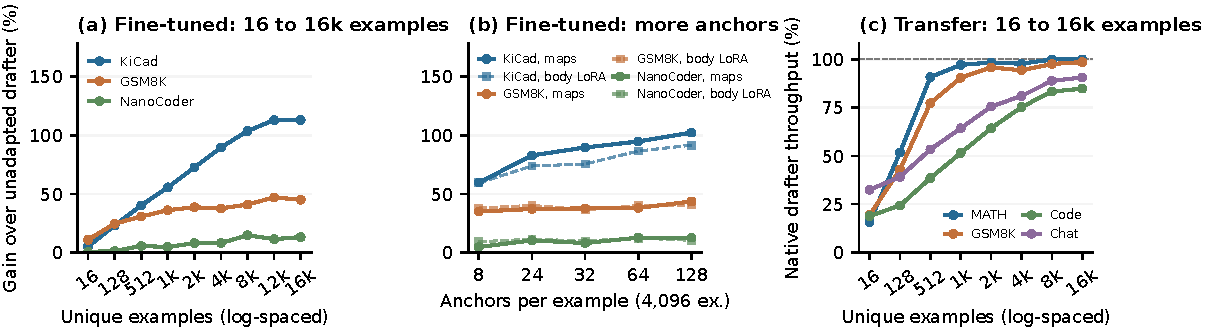
\includegraphics[width=\linewidth]{figures/relayspec_scaling.pdf}
    \caption{Supervision budget in both settings, from 16 to 16{,}384 training examples. (a) and (c) share a log-spaced example axis; (b) fixes examples at 4{,}096 and varies anchors per example. (a) and (b) use fine-tuned Qwen3-4B targets with the accept-until-fail objective, where solid lines train the five interface maps and dashed lines train a rank-128 LoRA inside the draft transformer. (c) transfers the Qwen3-4B drafter to Qwen3-8B with the reconstruction objective and plots throughput as a percentage of the native Qwen3-8B drafter. Adaptation is already effective at 16 examples and speedup keeps improving with supervision without saturating at the largest budget measured.}
    \label{fig:scaling}
\end{figure}


\subsection{EAGLE-3 recurrent objective}
\label{app:eagle-method}
\subsection{Extension to EAGLE-3}
\label{sec:method-eagle}
The construction is not specific to DFlash. EAGLE-3 combines features from three target layers before autoregressive drafting~\citep{li2025eagle3}, so $K=3$. We place one map before each of those inputs and leave the original feature projection, prediction network, and autoregressive drafting procedure unchanged. The maps fold into that projection exactly as in Equation~\ref{eq:folded-fusion}, so inference again runs the original architecture with one updated projection.

We pair each setting with the same objective we use for DFlash. For a LoRA-adapted target the feature widths match, so the maps start at the identity and receive token supervision. Because EAGLE-3 drafts one token at a time instead of filling a masked block, we apply the accept-until-fail rule along its own recurrent path. At each sampled anchor the drafter predicts up to eight successive tokens, a position is supervised only when every earlier prediction was correct, and the first incorrect prediction is still supervised. A saved token continues a path only where it matches the greedy prediction. The frozen drafter carries a reduced vocabulary head, so a target token outside that head ends a path without contributing a loss term, and we normalize each example by its own count of supervised positions. For a replaced target the widths can differ, so the maps start at Xavier-uniform values and train by reconstruction using Equation~\ref{eq:mse-method}.



\section{Complete analysis probe results}
\label{app:analysis-probes}

\makeatletter
\setlength{\@fptop}{0pt}
\setlength{\@fpsep}{12pt}
\setlength{\@fpbot}{0pt plus 1fil}
\makeatother
\renewcommand{\topfraction}{0.95}
\renewcommand{\bottomfraction}{0.95}
\renewcommand{\textfraction}{0.05}
\renewcommand{\floatpagefraction}{0.8}
\setcounter{topnumber}{6}
\setcounter{bottomnumber}{6}
\setcounter{totalnumber}{10}

This appendix reports the complete results for every probe cited in Section~\ref{sec:analysis}. It also reports several completed interventions that are not discussed in the main text. All results come from the Phase 1 and Phase 2 experimental reports. They were checked against the corresponding Markdown probe reports while preparing this appendix.

\subsection{LoRA-fine-tuned targets: direction and scale}
\label{app:lora-direction}

For each token position, let $z_0$ be the fused context without the learned maps and let $\delta$ be their learned correction. The dynamic intervention constructs $z_0+\delta_{\parallel}$ or $z_0+\delta_{\perp}$ before RMSNorm. Native and full dynamic controls use the same hook path. Every row in Table~\ref{tab:app-direction} uses the same 128 held-out prompts for its task.

\begin{table}[htbp]
\centering
\caption{Complete direction intervention results. Mean throughput is measured in tokens/s. Acceptance length $\tau$ is measured in tokens per verification step and includes the target contribution. Summed time is measured in seconds over 128 prompts. Gain and retained latency reduction are percentages relative to the matching dynamic controls.}
\label{tab:app-direction}
\small
\resizebox{\linewidth}{!}{%
\begin{tabular}{llrrrrr}
\toprule
Task & Context & Mean throughput & Gain & $\tau$ & Summed time & Retained latency reduction \\
\midrule
GSM8K & Native $z_0$ & 131.47 & 0.00\% & 4.472 & 149.636 & 0.0\% \\
GSM8K & Full $z_0+\delta$ & 180.17 & 37.05\% & 5.988 & 115.310 & 100.0\% \\
GSM8K & Parallel $z_0+\delta_{\parallel}$ & 124.61 & $-5.21\%$ & 4.466 & 157.729 & $-23.6\%$ \\
GSM8K & Perpendicular $z_0+\delta_{\perp}$ & 177.64 & 35.12\% & 5.924 & 117.436 & 93.8\% \\
NanoCoder & Native $z_0$ & 150.58 & 0.00\% & 5.111 & 191.998 & 0.0\% \\
NanoCoder & Full $z_0+\delta$ & 161.63 & 7.33\% & 5.552 & 182.780 & 100.0\% \\
NanoCoder & Parallel $z_0+\delta_{\parallel}$ & 150.78 & 0.13\% & 5.114 & 191.847 & 1.6\% \\
NanoCoder & Perpendicular $z_0+\delta_{\perp}$ & 170.39 & 13.15\% & 5.527 & 173.880 & 196.6\% \\
\bottomrule
\end{tabular}%
}
\end{table}

The NanoCoder timing ratio above 100\% is not evidence that the perpendicular component is functionally better than the full map. The full dynamic control saves only 9.218 seconds relative to its native dynamic control, while the perpendicular intervention saves 18.118 seconds in a separate measurement. The acceptance-length comparison is more stable and is the basis of the main-text interpretation.

The scaling probes use folded static projections. Correction strength $\alpha$ supplies $z_0+\alpha\delta$. Whole-context scaling instead supplies $2(z_0+\delta)$. Table~\ref{tab:app-scaling} includes the native and full endpoints, every tested correction strength, and the whole-context scaling control cited in Section~\ref{sec:analysis-lora}.

\begin{table}[htbp]
\centering
\caption{Complete correction-strength and whole-context scaling results. Mean throughput is measured in tokens/s. Acceptance length $\tau$ is measured in tokens per verification step. Gain and retained latency reduction are percentages relative to the matching static native and full controls.}
\label{tab:app-scaling}
\small
\resizebox{\linewidth}{!}{%
\begin{tabular}{llrrrr}
\toprule
Task & Static intervention & Mean throughput & Gain & $\tau$ & Retained latency reduction \\
\midrule
GSM8K & Native, $\alpha=0$ & 128.90 & 0.00\% & 4.472 & 0.0\% \\
GSM8K & Correction strength $0.5$ & 177.02 & 37.33\% & 5.757 & 98.9\% \\
GSM8K & Full, $\alpha=1$ & 179.83 & 39.51\% & 5.988 & 100.0\% \\
GSM8K & Correction strength $1.5$ & 175.61 & 36.24\% & 5.802 & 89.8\% \\
GSM8K & Correction strength $2$ & 165.93 & 28.72\% & 5.400 & 72.8\% \\
GSM8K & Whole context $\times 2$ & 181.07 & 40.47\% & 5.988 & 102.1\% \\
\midrule
NanoCoder & Native, $\alpha=0$ & 150.79 & 0.00\% & 5.111 & 0.0\% \\
NanoCoder & Correction strength $0.5$ & 169.23 & 12.23\% & 5.532 & 90.8\% \\
NanoCoder & Full, $\alpha=1$ & 171.73 & 13.89\% & 5.552 & 100.0\% \\
NanoCoder & Correction strength $1.5$ & 163.65 & 8.53\% & 5.321 & 54.0\% \\
NanoCoder & Correction strength $2$ & 152.46 & 1.11\% & 5.032 & $-4.4\%$ \\
NanoCoder & Whole context $\times 2$ & 166.34 & 10.32\% & 5.552 & 72.4\% \\
\bottomrule
\end{tabular}%
}
\end{table}

Whole-context doubling preserves the recorded acceptance length exactly on both tasks. Correction doubling does not. Relative to the full maps, mean throughput changes by $+0.69\%$ on GSM8K and $-3.14\%$ on NanoCoder. Acceptance length is a pooled ratio and does not determine each request's block schedule, output length, or token path. The variants were timed in separate, unrepeated passes, while scaling adds no inference operation. We therefore treat these small throughput differences as likely GPU timing variation rather than a causal speed effect.

\subsection{LoRA-shift geometry}
\label{app:lora-geometry}

The geometry probe teacher-forces identical saved tokens through the base target and the LoRA-fine-tuned target. It uses 64 cached training examples per task and 16 response positions per example, for 1,024 positions. Let $t$ be the fused-context change caused by LoRA fine-tuning and let $\delta$ be the map correction. The shuffled control randomly reassigns $t$ among sampled positions while leaving every correction fixed.

\begin{table}[ht!]
\centering
\caption{Complete LoRA-shift geometry results. Cosine similarity, radial energy fraction, and relative linearization error are dimensionless.}
\label{tab:app-lora-geometry}
\small
\resizebox{\linewidth}{!}{%
\begin{tabular}{lrrrrrr}
\toprule
Task & Positions & Mean cosine & Shuffled cosine & Difference & Radial energy & RMSNorm error \\
\midrule
GSM8K & 1,024 & $-0.0429$ & $-0.0413$ & $-0.0016$ & 25.22\% & 17.55\% \\
NanoCoder & 1,024 & 0.1248 & 0.1052 & 0.0195 & 34.82\% & 14.88\% \\
\bottomrule
\end{tabular}%
}
\end{table}

Radial energy is the fraction of $\sum_p\|\delta_p\|^2$ parallel to $z_{0,p}$. RMSNorm error is the norm of the difference between the full normalized change and its first-order approximation, divided by the norm of the full normalized change. Neither quantity is an acceptance or speed measurement.

\subsection{Qwen3-4B drafter to Qwen3-8B target: feature reconstruction}
\label{app:transfer-geometry}

The feature probe uses 64 training records and 7,090 sampled positions, split into 2,994 prompt and 4,096 response positions. Feature and context errors are normalized squared errors and are dimensionless. Context error is measured after frozen fusion and RMSNorm. Source cosine is the dimensionless cosine similarity between a mapped 8B feature and its paired 4B feature. The MSE, AUF, and decay rows are complete training recipes with different learning rates and supervision coverage.

\begin{table}[ht!]
\centering
\caption{Complete fused-context reconstruction results. Errors are dimensionless normalized squared errors. Lower is better.}
\label{tab:app-context-geometry}
\small
\begin{tabular}{lrr}
\toprule
Recipe & Prompt context error & Response context error \\
\midrule
MSE & 0.216170 & 0.136147 \\
AUF & 1.228544 & 0.940413 \\
Decay CE & 1.189191 & 0.899731 \\
\bottomrule
\end{tabular}
\end{table}

\begin{table}[htbp]
\centering
\caption{Complete per-layer feature reconstruction results. Feature error is a dimensionless normalized squared error, and source cosine is dimensionless. P and R denote prompt and response positions. Layer numbers index the five feature streams in RelaySpec.}
\label{tab:app-layer-geometry}
\scriptsize
\setlength{\tabcolsep}{2pt}
\begin{minipage}[t]{0.48\linewidth}
\vspace{0pt}
\centering
\textbf{MSE}\par\smallskip
\begin{tabular}{@{}rrrrr@{}}
\toprule
Layer & P error & R error & P cosine & R cosine \\
\midrule
0 & 0.060359 & 0.033437 & 0.975595 & 0.984793 \\
1 & 0.191632 & 0.068966 & 0.899016 & 0.965129 \\
2 & 0.192591 & 0.083779 & 0.901045 & 0.957394 \\
3 & 0.191474 & 0.110141 & 0.902611 & 0.944060 \\
4 & 0.180501 & 0.090359 & 0.909023 & 0.954783 \\
\bottomrule
\end{tabular}
\end{minipage}\hfill
\begin{minipage}[t]{0.48\linewidth}
\vspace{0pt}
\centering
\textbf{AUF}\par\smallskip
\begin{tabular}{@{}rrrrr@{}}
\toprule
Layer & P error & R error & P cosine & R cosine \\
\midrule
0 & 2.742802 & 2.794326 & 0.195425 & 0.214868 \\
1 & 2.859036 & 2.540209 & 0.112855 & 0.120631 \\
2 & 21.592222 & 12.066430 & 0.141729 & 0.175011 \\
3 & 6.882195 & 4.716092 & 0.144134 & 0.226237 \\
4 & 3.814032 & 3.408715 & 0.190191 & 0.266906 \\
\bottomrule
\end{tabular}
\end{minipage}
\par\smallskip
\begin{minipage}[t]{0.48\linewidth}
\vspace{0pt}
\centering
\textbf{Decay CE}\par\smallskip
\begin{tabular}{@{}rrrrr@{}}
\toprule
Layer & P error & R error & P cosine & R cosine \\
\midrule
0 & 2.710681 & 2.753600 & 0.201154 & 0.220411 \\
1 & 2.827380 & 2.522013 & 0.119284 & 0.126873 \\
2 & 21.544376 & 12.034999 & 0.145896 & 0.179880 \\
3 & 6.830830 & 4.675968 & 0.151039 & 0.234286 \\
4 & 3.730459 & 3.298069 & 0.201127 & 0.278744 \\
\bottomrule
\end{tabular}
\end{minipage}
\end{table}

\subsection{Held-out common-input diagnostics}
\label{app:heldout-diagnostics}

For each workload, the probe selects eight held-out responses and eight identical test positions per response, for 64 tests per variant. At each position, the frozen drafter predicts the next 15 tokens from the saved response. Full cross-entropy is measured in nats per predicted token. AUF support is the percentage of valid tokens that would receive AUF loss. Correct prefix is the mean number of consecutive correct predictions before the first error and is measured in tokens. Prompt and response errors are dimensionless normalized context errors. These offline prefixes are not live acceptance lengths.

\begin{table}[htbp]
\centering
\caption{Complete held-out MATH diagnostics. Cross-entropy is in nats/token, AUF support is a percentage, correct prefix is in tokens, and context errors are dimensionless.}
\label{tab:app-heldout-math}
\scriptsize
\begin{tabular}{lrrrrr}
\toprule
Variant & Cross-entropy & AUF support & Correct prefix & Prompt error & Response error \\
\midrule
MSE & 1.6939 & 51.81\% & 6.7656 & 0.1821 & 0.1236 \\
Decay midpoint & 1.8043 & 49.79\% & 6.4844 & 0.7590 & 0.4928 \\
Decay CE & 1.9534 & 47.13\% & 6.0625 & 1.3852 & 0.9058 \\
Warm unseen 4k & 2.0634 & 52.45\% & 6.9219 & 0.3910 & 0.3867 \\
Warm seen 4k & 2.0695 & 50.64\% & 6.6094 & 0.3947 & 0.3827 \\
AUF midpoint & 2.1282 & 48.51\% & 6.2812 & 0.7768 & 0.5110 \\
Warm unseen 8k & 2.1507 & 54.47\% & 7.2188 & 0.4347 & 0.4084 \\
Warm seen 8k & 2.1760 & 56.49\% & 7.5625 & 0.4362 & 0.4088 \\
AUF & 2.6028 & 45.74\% & 5.8438 & 1.4131 & 0.9333 \\
Random initial & 8.6261 & 6.81\% & 0.0000 & 4.4041 & 4.9689 \\
\bottomrule
\end{tabular}
\par\medskip
\caption{Complete held-out GSM8K diagnostics. Units match Table~\ref{tab:app-heldout-math}.}
\label{tab:app-heldout-gsm}
\begin{tabular}{lrrrrr}
\toprule
Variant & Cross-entropy & AUF support & Correct prefix & Prompt error & Response error \\
\midrule
Decay midpoint & 1.5407 & 55.01\% & 7.1875 & 0.7967 & 0.4933 \\
Decay CE & 1.6564 & 50.70\% & 6.5312 & 1.4673 & 0.8850 \\
Warm seen 4k & 1.7356 & 50.91\% & 6.5625 & 0.4074 & 0.3686 \\
Warm seen 8k & 1.7586 & 57.48\% & 7.5781 & 0.4506 & 0.3911 \\
Warm unseen 8k & 1.7793 & 55.65\% & 7.3125 & 0.4535 & 0.3911 \\
MSE & 1.7817 & 53.07\% & 6.8750 & 0.2026 & 0.1146 \\
Warm unseen 4k & 1.8745 & 55.65\% & 7.2812 & 0.4053 & 0.3692 \\
AUF midpoint & 1.9572 & 55.76\% & 7.3125 & 0.8212 & 0.5098 \\
AUF & 2.0566 & 54.14\% & 7.0781 & 1.5231 & 0.9074 \\
Random initial & 9.6898 & 7.00\% & 0.0156 & 4.0335 & 4.6817 \\
\bottomrule
\end{tabular}
\par\medskip
\caption{Complete held-out Code diagnostics. Units match Table~\ref{tab:app-heldout-math}.}
\label{tab:app-heldout-code}
\begin{tabular}{lrrrrr}
\toprule
Variant & Cross-entropy & AUF support & Correct prefix & Prompt error & Response error \\
\midrule
MSE & 2.6039 & 40.46\% & 4.8750 & 0.3942 & 0.2864 \\
Warm unseen 4k & 3.4776 & 32.24\% & 3.6719 & 0.5446 & 0.4510 \\
Warm unseen 8k & 3.5000 & 32.79\% & 3.7344 & 0.5785 & 0.4877 \\
Warm seen 8k & 3.5864 & 32.02\% & 3.6250 & 0.5754 & 0.4818 \\
Warm seen 4k & 3.6100 & 33.77\% & 3.8906 & 0.5456 & 0.4543 \\
Decay midpoint & 3.7045 & 25.33\% & 2.6406 & 0.9133 & 0.6970 \\
AUF midpoint & 4.1200 & 28.62\% & 3.1250 & 0.9301 & 0.7159 \\
Decay CE & 4.6468 & 17.98\% & 1.5625 & 1.5436 & 1.2464 \\
AUF & 5.5081 & 17.00\% & 1.4219 & 1.5820 & 1.2868 \\
Random initial & 9.8854 & 7.24\% & 0.0312 & 3.7889 & 4.6308 \\
\bottomrule
\end{tabular}
\par\medskip
\caption{Complete held-out Chat diagnostics. Units match Table~\ref{tab:app-heldout-math}.}
\label{tab:app-heldout-chat}
\begin{tabular}{lrrrrr}
\toprule
Variant & Cross-entropy & AUF support & Correct prefix & Prompt error & Response error \\
\midrule
MSE & 3.8074 & 28.50\% & 2.9062 & 0.3017 & 0.3255 \\
Warm unseen 8k & 4.1924 & 26.64\% & 2.6406 & 0.4872 & 0.4895 \\
Warm seen 4k & 4.2015 & 26.99\% & 2.6719 & 0.4507 & 0.4547 \\
Warm seen 8k & 4.2630 & 24.65\% & 2.3594 & 0.4868 & 0.4873 \\
Warm unseen 4k & 4.2904 & 24.42\% & 2.3281 & 0.4504 & 0.4519 \\
Decay midpoint & 4.5984 & 21.03\% & 1.8750 & 0.9437 & 0.7632 \\
AUF midpoint & 4.9769 & 22.78\% & 2.1094 & 0.9668 & 0.7841 \\
Decay CE & 5.6398 & 16.36\% & 1.2188 & 1.7617 & 1.3749 \\
AUF & 6.2094 & 13.55\% & 0.8438 & 1.8059 & 1.4210 \\
Random initial & 10.7415 & 7.48\% & 0.0000 & 4.9159 & 4.0375 \\
\bottomrule
\end{tabular}
\end{table}

\FloatBarrier
\subsection{Complete live midpoint intervention}
\label{app:midpoint-full}

For each token-trained parent, the midpoint averages all five parent maps with the corresponding MSE maps. There is no retraining. Each endpoint uses 128 prompts. Mean and pooled throughput are measured in tokens/s. Acceptance length is measured in tokens per verification step. Total time is measured in seconds. Native and parent comparisons are shown with multiplication signs. Latency reduction is a percentage relative to the named cold parent. Endpoints were timed in separate passes.

\begin{table}[htbp]
\centering
\caption{All parent, midpoint, and MSE endpoints in the live interpolation probe.}
\label{tab:app-midpoint}
\scriptsize
\resizebox{\linewidth}{!}{%
\begin{tabular}{lllrrrrrrr}
\toprule
Task & Parent & Variant & Mean throughput & Pooled throughput & Native ratio & Parent ratio & Total time & Latency reduction & $\tau$ \\
\midrule
Code & AUF & MSE & 126.18 & 124.01 & $0.8322\times$ & $2.1618\times$ & 569.96 & 50.08\% & 4.6912 \\
Code & AUF & Midpoint & 81.64 & 85.41 & $0.5384\times$ & $1.3986\times$ & 827.50 & 27.53\% & 3.2512 \\
Code & AUF & Parent & 58.37 & 61.90 & $0.3850\times$ & $1.0000\times$ & 1141.85 & 0.00\% & 2.3456 \\
Code & Decay CE & MSE & 126.18 & 124.01 & $0.8322\times$ & $2.0498\times$ & 569.96 & 47.75\% & 4.6912 \\
Code & Decay CE & Midpoint & 84.68 & 88.03 & $0.5585\times$ & $1.3756\times$ & 802.88 & 26.39\% & 3.3368 \\
Code & Decay CE & Parent & 61.56 & 64.80 & $0.4060\times$ & $1.0000\times$ & 1090.76 & 0.00\% & 2.4489 \\
MATH & AUF & MSE & 219.48 & 216.72 & $0.9986\times$ & $1.1300\times$ & 406.20 & 13.83\% & 7.9776 \\
MATH & AUF & Midpoint & 206.81 & 201.87 & $0.9410\times$ & $1.0648\times$ & 436.09 & 7.48\% & 7.5624 \\
MATH & AUF & Parent & 194.22 & 186.76 & $0.8837\times$ & $1.0000\times$ & 471.37 & 0.00\% & 6.8923 \\
MATH & Decay CE & MSE & 219.48 & 216.72 & $0.9986\times$ & $1.1273\times$ & 406.20 & 13.39\% & 7.9776 \\
MATH & Decay CE & Midpoint & 208.80 & 203.73 & $0.9500\times$ & $1.0725\times$ & 432.11 & 7.86\% & 7.5748 \\
MATH & Decay CE & Parent & 194.69 & 187.71 & $0.8858\times$ & $1.0000\times$ & 468.98 & 0.00\% & 6.9474 \\
\bottomrule
\end{tabular}%
}
\end{table}

\FloatBarrier
\subsection{Complete warm AUF refinement results}
\label{app:warm-full}

All four refinements start from the same 8k MSE parent and run AUF for three epochs. Seen data overlap the MSE training examples. Unseen data are disjoint from them. Mean throughput is measured in tokens/s. Acceptance length is measured in tokens per verification step. Fit time is measured in minutes and includes the MSE parent and AUF stage.

\begin{table}[htbp]
\centering
\caption{All 16 warm-refinement endpoints. Native and MSE-parent throughput ratios use multiplication signs. Latency reduction is a percentage relative to native.}
\label{tab:app-warm}
\scriptsize
\begin{tabular}{llrrrrrr}
\toprule
Task & AUF data & Native ratio & MSE-parent ratio & Mean throughput & Latency reduction & $\tau$ & Fit time \\
\midrule
Chat & Unseen 4k & $0.8548\times$ & $0.9624\times$ & 76.51 & $-17.33\%$ & 2.7495 & 32.39 \\
Chat & Seen 8k & $0.8446\times$ & $0.9509\times$ & 75.59 & $-19.06\%$ & 2.7038 & 45.32 \\
Chat & Unseen 8k & $0.8431\times$ & $0.9492\times$ & 75.46 & $-19.32\%$ & 2.7030 & 47.42 \\
Chat & Seen 4k & $0.8420\times$ & $0.9480\times$ & 75.36 & $-18.58\%$ & 2.7403 & 31.52 \\
Code & Unseen 4k & $0.7417\times$ & $0.8913\times$ & 112.46 & $-26.52\%$ & 4.3499 & 32.39 \\
Code & Seen 4k & $0.7273\times$ & $0.8740\times$ & 110.28 & $-27.86\%$ & 4.2769 & 31.52 \\
Code & Unseen 8k & $0.7051\times$ & $0.8473\times$ & 106.92 & $-31.27\%$ & 4.1818 & 47.42 \\
Code & Seen 8k & $0.7043\times$ & $0.8463\times$ & 106.78 & $-32.01\%$ & 4.1525 & 45.32 \\
GSM8K & Unseen 8k & $1.0606\times$ & $1.0874\times$ & 188.72 & 5.53\% & 6.6218 & 47.42 \\
GSM8K & Seen 8k & $1.0431\times$ & $1.0696\times$ & 185.62 & 3.50\% & 6.5891 & 45.32 \\
GSM8K & Unseen 4k & $1.0413\times$ & $1.0677\times$ & 185.30 & 4.01\% & 6.5340 & 32.39 \\
GSM8K & Seen 4k & $1.0339\times$ & $1.0601\times$ & 183.97 & 3.40\% & 6.4951 & 31.52 \\
MATH & Seen 8k & $0.9927\times$ & $0.9941\times$ & 218.18 & $-1.32\%$ & 7.8662 & 45.32 \\
MATH & Unseen 8k & $0.9911\times$ & $0.9925\times$ & 217.82 & $-1.83\%$ & 7.8410 & 47.42 \\
MATH & Seen 4k & $0.9717\times$ & $0.9731\times$ & 213.57 & $-3.20\%$ & 7.8145 & 31.52 \\
MATH & Unseen 4k & $0.9694\times$ & $0.9707\times$ & 213.05 & $-3.42\%$ & 7.7785 & 32.39 \\
\bottomrule
\end{tabular}
\end{table}

The warm runs improve GSM8K and weaken MATH, Code, and Chat relative to the MSE parent. This pattern is consistent with workload-specific refinement, but it does not establish overfitting because matched training and held-out learning curves were not recorded.

\subsection{Rectangular-identity initialization}
\label{app:identity-init}

This probe repeats the T1 8k MSE, AUF, and decaying-cross-entropy fits from a rectangular identity. Each map initially copies the first 2,560 coordinates of the 4,096-dimensional 8B feature and sets the remaining input directions to zero. Corresponding coordinates need not have the same meaning in the two models. All three retries use 8,192 training examples, three epochs, and learning rate $10^{-3}$. The fusion projection, normalization, embeddings, vocabulary head, and drafter transformer remain frozen.

For MSE, the original and retry both use learning rate $10^{-3}$, so their only planned recipe change is map initialization. The original AUF and decay fits use Xavier initialization and learning rate $10^{-4}$. Their retries change both initialization and learning rate. Their improvements cannot be assigned to either change alone.

\begin{table}[htbp]
\centering
\caption{Complete rectangular-identity endpoints. Mean throughput is measured in tokens/s. Acceptance length $\tau$ is measured in tokens per verification step. Native throughput ratios are shown with multiplication signs. Each workload uses 128 prompts.}
\label{tab:app-identity-endpoints}
\small
\begin{tabular}{llrrr}
\toprule
Workload & Recipe & Mean throughput & Native ratio & $\tau$ \\
\midrule
MATH & MSE & 213.70 & $0.9723\times$ & 7.983 \\
MATH & AUF & 206.16 & $0.9380\times$ & 7.326 \\
MATH & Decay CE & 203.74 & $0.9270\times$ & 7.348 \\
GSM8K & MSE & 166.70 & $0.9368\times$ & 6.217 \\
GSM8K & AUF & 175.35 & $0.9854\times$ & 6.166 \\
GSM8K & Decay CE & 169.72 & $0.9538\times$ & 6.073 \\
Code & MSE & 119.49 & $0.7881\times$ & 4.569 \\
Code & AUF & 73.10 & $0.4821\times$ & 2.931 \\
Code & Decay CE & 76.02 & $0.5014\times$ & 3.042 \\
Chat & MSE & 76.13 & $0.8506\times$ & 2.747 \\
Chat & AUF & 60.77 & $0.6790\times$ & 2.163 \\
Chat & Decay CE & 61.11 & $0.6828\times$ & 2.183 \\
\bottomrule
\end{tabular}
\end{table}

\begin{table}[htbp]
\centering
\caption{Complete comparison with the original Xavier-initialized fits. Throughput columns are measured in tokens/s. Acceptance length columns are measured in tokens per verification step. Changes are percentages relative to the original fit.}
\label{tab:app-identity-change}
\scriptsize
\begin{tabular}{llrrrrrr}
\toprule
Workload & Recipe & Original throughput & Identity throughput & Change & Original $\tau$ & Identity $\tau$ & Change \\
\midrule
MATH & MSE & 218.75 & 213.70 & $-2.31\%$ & 7.973 & 7.983 & $+0.14\%$ \\
MATH & AUF & 194.22 & 206.16 & $+6.15\%$ & 6.892 & 7.326 & $+6.29\%$ \\
MATH & Decay CE & 194.69 & 203.74 & $+4.65\%$ & 6.947 & 7.348 & $+5.77\%$ \\
GSM8K & MSE & 172.35 & 166.70 & $-3.28\%$ & 6.204 & 6.217 & $+0.21\%$ \\
GSM8K & AUF & 162.05 & 175.35 & $+8.21\%$ & 5.677 & 6.166 & $+8.60\%$ \\
GSM8K & Decay CE & 163.47 & 169.72 & $+3.82\%$ & 5.693 & 6.073 & $+6.68\%$ \\
Code & MSE & 125.98 & 119.49 & $-5.15\%$ & 4.690 & 4.569 & $-2.58\%$ \\
Code & AUF & 58.37 & 73.10 & $+25.24\%$ & 2.346 & 2.931 & $+24.94\%$ \\
Code & Decay CE & 61.56 & 76.02 & $+23.49\%$ & 2.449 & 3.042 & $+24.20\%$ \\
Chat & MSE & 78.31 & 76.13 & $-2.78\%$ & 2.802 & 2.747 & $-1.94\%$ \\
Chat & AUF & 49.93 & 60.77 & $+21.73\%$ & 1.767 & 2.163 & $+22.41\%$ \\
Chat & Decay CE & 51.31 & 61.11 & $+19.09\%$ & 1.812 & 2.183 & $+20.52\%$ \\
\bottomrule
\end{tabular}
\end{table}

\begin{table}[htbp]
\centering
\caption{Rectangular-identity fitting cost. Wall time is measured in minutes. GPU time is measured in GPU-hours on two GPUs.}
\label{tab:app-identity-fit}
\small
\begin{tabular}{lrr}
\toprule
Recipe & Wall time & GPU time \\
\midrule
MSE & 11.11 & 0.370 \\
AUF & 30.14 & 1.005 \\
Decay CE & 29.54 & 0.985 \\
\bottomrule
\end{tabular}
\end{table}

\FloatBarrier
MSE retains the highest acceptance length on all four workloads and the highest measured throughput on MATH, Code, and Chat. AUF is faster on GSM8K in this single pass despite having a slightly lower acceptance length. There are no repeated timing trials, so this disagreement does not establish a stable throughput advantage or timing noise. The MSE initializer-only comparison supports retaining the selected Xavier initialization. The token-recipe retries show that their original initialization and learning rate are not the only settings under which they can learn, but do not isolate which change helped.

\clearpage
\subsection{Additional completed probes not used in the main analysis}
\label{app:additional-probes}

The following completed probes informed the decision to keep the main analysis narrow. They are reported here so negative and secondary results remain visible.

\subsubsection{Removing one map correction}

Removing map $i$ replaces $W_i$ with the identity and leaves its native feature stream and fusion block in place. Map indices 0 through 4 correspond to target layers 1, 9, 17, 25, and 33. Throughput is measured in tokens/s. Acceptance length is measured in tokens per verification step.

\begin{table}[htbp]
\centering
\caption{Complete single-map removal results. Gain and retained latency reduction are percentages relative to the static controls.}
\label{tab:app-map-removal}
\small
\begin{tabular}{llrrrr}
\toprule
Task & Removed map & Mean throughput & Gain & $\tau$ & Retained latency reduction \\
\midrule
GSM8K & 0 & 174.69 & 35.52\% & 5.982 & 88.6\% \\
GSM8K & 1 & 178.72 & 38.65\% & 5.979 & 97.9\% \\
GSM8K & 2 & 184.68 & 43.27\% & 6.006 & 109.6\% \\
GSM8K & 3 & 176.18 & 36.68\% & 5.908 & 94.9\% \\
GSM8K & 4 & 171.68 & 33.18\% & 5.833 & 86.4\% \\
NanoCoder & 0 & 167.18 & 10.87\% & 5.577 & 74.9\% \\
NanoCoder & 1 & 170.44 & 13.03\% & 5.569 & 90.6\% \\
NanoCoder & 2 & 170.78 & 13.26\% & 5.587 & 92.9\% \\
NanoCoder & 3 & 170.51 & 13.08\% & 5.539 & 92.8\% \\
NanoCoder & 4 & 168.31 & 11.62\% & 5.447 & 84.9\% \\
\bottomrule
\end{tabular}
\end{table}

\subsubsection{Using maps trained for another LoRA-fine-tuned target}

The evaluated target, target LoRA, and prompts remain fixed while the complete five-map bank is replaced. No completed KiCad destination comparison is available.

\begin{table}[ht!]
\centering
\caption{Complete foreign-bank results. Throughput is measured in tokens/s. Acceptance length $\tau$ is measured in tokens per verification step. Gain and retained latency reduction are percentages relative to the destination task's native and full controls.}
\label{tab:app-bank-swap}
\small
\begin{tabular}{llrrrr}
\toprule
Destination & Source bank & Mean throughput & Gain & $\tau$ & Retained latency reduction \\
\midrule
GSM8K & KiCad & 127.63 & $-0.99\%$ & 4.430 & $-2.5\%$ \\
GSM8K & NanoCoder & 129.72 & 0.63\% & 4.565 & 4.2\% \\
NanoCoder & GSM8K & 148.97 & $-1.20\%$ & 5.016 & $-2.0\%$ \\
NanoCoder & KiCad & 148.12 & $-1.77\%$ & 4.990 & $-11.1\%$ \\
\bottomrule
\end{tabular}
\end{table}

\subsubsection{Low-rank correction probes}

Whole-map truncation applies SVD to $W_i$ and removes most of the identity path. Correction truncation applies SVD only to $W_i-I$ and then restores the identity. Every reported rank is per map. All exports still use a dense folded projection, so these measurements do not demonstrate a low-rank inference-speed benefit.

\begin{table}[htbp]
\centering
\caption{Complete first-pass low-rank results. Throughput is measured in tokens/s. Acceptance length $\tau$ is measured in tokens per verification step. Gain and retained latency reduction are percentages relative to static controls.}
\label{tab:app-rank-first}
\scriptsize
\begin{tabular}{lllrrrr}
\toprule
Task & Truncated object & Rank & Mean throughput & Gain & $\tau$ & Retained latency reduction \\
\midrule
GSM8K & Whole map & 1 & 34.16 & $-73.50\%$ & 1.145 & $-1142.5\%$ \\
GSM8K & Whole map & 2 & 34.50 & $-73.24\%$ & 1.165 & $-1125.0\%$ \\
GSM8K & Correction & 1 & 143.26 & 11.14\% & 4.913 & 36.9\% \\
GSM8K & Correction & 2 & 148.99 & 15.58\% & 5.072 & 49.6\% \\
GSM8K & Correction & 64 & 172.81 & 34.06\% & 5.931 & 87.6\% \\
GSM8K & Correction & 128 & 179.10 & 38.94\% & 5.928 & 99.2\% \\
GSM8K & Correction & 256 & 172.59 & 33.89\% & 5.964 & 87.0\% \\
NanoCoder & Whole map & 1 & 31.06 & $-79.40\%$ & 1.057 & $-3484.4\%$ \\
NanoCoder & Whole map & 2 & 33.06 & $-78.08\%$ & 1.076 & $-3248.1\%$ \\
NanoCoder & Correction & 1 & 157.11 & 4.19\% & 5.239 & 38.8\% \\
NanoCoder & Correction & 2 & 151.77 & 0.65\% & 5.259 & 2.1\% \\
NanoCoder & Correction & 128 & 163.60 & 8.50\% & 5.492 & 60.1\% \\
NanoCoder & Correction & 256 & 168.04 & 11.44\% & 5.521 & 83.1\% \\
NanoCoder & Correction & 512 & 167.20 & 10.89\% & 5.528 & 76.2\% \\
NanoCoder & Correction & 1,024 & 168.84 & 11.97\% & 5.546 & 84.5\% \\
NanoCoder & Correction & 2,048 & 166.49 & 10.41\% & 5.553 & 72.3\% \\
\bottomrule
\end{tabular}
\end{table}

\begin{table}[htbp]
\centering
\caption{Complete repeated timing results for selected correction ranks. Throughput is measured in tokens/s. Acceptance length $\tau$ is measured in tokens per verification step. Gain and retained latency reduction are percentages relative to the native and full controls from the same repeat.}
\label{tab:app-rank-repeats}
\scriptsize
\begin{tabular}{llrrrr}
\toprule
Task and repeat & Variant & Mean throughput & Gain & $\tau$ & Retained latency reduction \\
\midrule
GSM8K, repeat 0 & Native & 124.91 & 0.00\% & 4.472 & 0.0\% \\
GSM8K, repeat 0 & Full & 176.03 & 40.92\% & 5.988 & 100.0\% \\
GSM8K, repeat 0 & Correction rank 128 & 172.81 & 38.35\% & 5.928 & 95.1\% \\
GSM8K, repeat 0 & Correction rank 256 & 180.10 & 44.18\% & 5.964 & 106.7\% \\
GSM8K, repeat 1 & Native & 127.34 & 0.00\% & 4.472 & 0.0\% \\
GSM8K, repeat 1 & Full & 184.00 & 44.50\% & 5.988 & 100.0\% \\
GSM8K, repeat 1 & Correction rank 128 & 183.07 & 43.76\% & 5.928 & 99.6\% \\
GSM8K, repeat 1 & Correction rank 256 & 176.10 & 38.29\% & 5.964 & 88.6\% \\
NanoCoder, repeat 0 & Native & 152.44 & 0.00\% & 5.111 & 0.0\% \\
NanoCoder, repeat 0 & Full & 171.03 & 12.20\% & 5.552 & 100.0\% \\
NanoCoder, repeat 0 & Correction rank 256 & 163.49 & 7.25\% & 5.521 & 57.8\% \\
NanoCoder, repeat 0 & Correction rank 512 & 166.52 & 9.24\% & 5.528 & 72.4\% \\
NanoCoder, repeat 1 & Native & 157.04 & 0.00\% & 5.111 & 0.0\% \\
NanoCoder, repeat 1 & Full & 172.93 & 10.12\% & 5.552 & 100.0\% \\
NanoCoder, repeat 1 & Correction rank 256 & 171.45 & 9.18\% & 5.521 & 89.3\% \\
NanoCoder, repeat 1 & Correction rank 512 & 166.80 & 6.22\% & 5.528 & 52.1\% \\
\bottomrule
\end{tabular}
\end{table}


\end{document}
